\documentclass[draftthesis,tocnosub,noragright,centerchapter,fullpagesingle,12pt]{uiuc_csthesis21}
\makeatletter
\usepackage{setspace}  % Useful for single, 1.5, and double spacing
\usepackage[numbers, sort]{natbib}  % Useful for formatting reference section
\usepackage{url}  % Useful for URLs
\usepackage{hyperref}  % Another package useful for URL
\usepackage{lscape} 
\def\fillandplacepagenumber{
	\par
	\pagestyle{empty}
	\vbox to 0pt{\vss}
	\vfill
	\vbox to 0pt{
		\baselineskip 0pt
		\hbox to \linewidth{\hss}
		\baselineskip\footskip
		\hbox to \linewidth{\hfil\thepage\hfil}\vss
	}
}

\usepackage{graphicx}  % Please import figures that are *high resolution* PDFs
\usepackage{epsfig}   % or EPS files
\usepackage{caption}
\usepackage{makecell}
\usepackage{algorithmic}
\usepackage{chronology}
\usepackage{subfigure}  % Useful for subfigures
\usepackage{subcaption}  % Useful for captioning subfigures
\usepackage{booktabs}  
\usepackage{multicol}
\usepackage{multirow}
\usepackage{amsfonts}
\usepackage{amsmath}
\usepackage{amssymb}
\usepackage{amstext}
\usepackage{amsthm}
\usepackage{algpseudocode}
\usepackage{algorithm}
\DeclareMathOperator*{\minimize}{minimize}
\DeclareMathOperator*{\maximize}{maximize}
\theoremstyle{definition}
\newtheorem{definition}{Definition}[chapter]
\newtheorem{lemma}{Lemma}[chapter]
\newtheorem{theorem}{Theorem}[chapter]
\newtheorem{corollary}{Corollary}[chapter]
\newtheorem{conjecture}{Conjecture}[chapter]
\newtheorem{remark}{Remark}[chapter]
\renewcommand{\qedsymbol}{QED.}  
\renewcommand{\algorithmicrequire}{\textbf{Input:}}
\renewcommand{\algorithmicensure}{\textbf{Output:}}
\usepackage{listings} 
\usepackage[ruled]{algorithm2e} 
\numberwithin{algocf}{chapter}
\phdthesis
\title{Efficient and Robust Web Scale Retrieval, Generation and Understanding}
\author{Daniel Campos}
\department{Computer Science}
\degreeyear{2023}
\advisor{Cheng Xiang Zhai }
\committee{Cheng Xiang Zhai, (UIUC, Chair)  \\
Alessandro Magnani (WalmartLabs, External Member) \\
Jiawei Han (UIUC)\\
Kevin Chang (UIUC)}
\begin{document}
\maketitle
\parindent 1em%

\frontmatter
\begin{abstract}
Large language models (LLM) effectively represent contextualized word representations across languages, domains, and tasks. Drive by these abilities; these models have become a building staple for many researchers and engineers who use text as their medium of representation, much like concrete is a staple in the construction world. Via the broad study and implementation, problems with large models have come to light: they can be expensive, brittle to noise, and produce unwanted outputs. Their large size and computational overhead make them difficult and expensive to deploy and use for inference. Minor variations in text inputs, such as typos or misspellings, can cause major losses in model accuracy. Seeking to improve how these models can be used for \textit{real world} usage and deployments, this thesis focuses on framing model used as a modular approach as model portions can be compressed, hardened, and optimized to deployment needs. To explore the challenges with large-scale deployments concerning robustness and inference efficiency, we explore four commonly used language workloads: textual understanding and classification, passage retrieval, text generation, and audio transcription generation. We chose these broad but connected tasks to ensure that our compression approaches broadly apply to natural language processing. First, we propose a general framework for improving model inference on broad language understanding workloads by studying how methods like unstructured pruning, structured pruning, and quantization can be leveraged to compress models and improve inference speeds. In studying compression for language understanding, we demonstrate that sparse language models can transfer to novel domains and tasks without further optimization. These sparse models can be combined with quantization and structured pruning to deliver massive speed-ups for minor losses in accuracy. Second, we study how leveraging multi-task modeling, knowledge distillation, and quantization can be leveraged to enable web-scale labeling of customer feedback. Using multi-task learning, task-specific knowledge, and model quantization, we can decrease the overall inference cost by 44\% for a major customer experience management company.  Third, we explore methods of tuning and optimizing dense retrieval methods post-training to ensure they perform well on real-world data. Our experiments yield simple and effective methods of increasing model robustness and decreasing inference costs without any need for retraining or index re-generation. Finally, we discuss our future work, which focuses on sequential compression approaches to sequence LLMs to allow generative workloads to reach web-scale deployments.
\end{abstract}
\tableofcontents
\mainmatter
\chapter{Introduction}
\label{chp:intro}
\section{Background}
Computers and computational devices have long been improving how humans think and act. At first, using a computer required large rooms of specialized equipment and expert operators. Since then, decades of gradual improvements led to the proliferation of cell phones and virtual supercomputers, which reside in the pockets of billions of people around the globe. These ubiquitous computing devices have become the interface that has brought the world into a truly connected mesh interface. Sharing one's daily experiences with thousands of viewers worldwide with little or no delay is not only possible but as common as driving a car. \\
In the world of artificial intelligence and natural language processing, there have also been decades of continuous improvement, which have led to models which can do truly impressive feats. Decades ago, it seemed far-fetched that one could ask a system obscure questions and receive the correct answer. Not only can this be done, but questions can come in spoken language, and responses sound natural despite their technological origin. \\
While personal computing devices can empower incredible experiences, most processing does not happen on devices. Instead, most of the \textit{work} happens in large data centers where economies of scale allow for cost-effective and failure-resistant infrastructure. Using customized deployments, services assemble their experiences by customizing complex workflows and experiences given their customer needs and constraints. \\
While all data center/cloud workloads are growing, those leveraging large neural network models have seen explosive growth. Models have grown from millions of parameters \cite{Krizhevsky2012ImageNetCW} to billions of \cite{Brown2020LanguageMA} and will likely reach trillions \cite{Fedus2021SwitchTS}. Despite the eye-catching model size growth, the bigger driver of computing is the widespread adoption of these models. In the earlier part of the 2010s, few companies were training AI models, and even fewer were using them. In 2022 79\% of companies had at least 3 models in production, up 17\% from a year before \footnote{https://www2.deloitte.com/us/en/pages/consulting/articles/state-of-ai-2022.html} \footnote{https://www2.deloitte.com/us/en/pages/about-deloitte/articles/press-releases/deloitte-state-of-ai-fourth-edition-report.html}. \\
In natural language processing, major advances have been driven by the proliferation of large models. One of the major goals of natural language processing is to understand human language in all its intricacies and uniqueness. Word representations created by using large textual corpora like GLoVE \cite{Pennington2014GloVeGV} and Word2Vec \cite{Mikolov2013DistributedRO} allowed for major improvements in tasks like sentiment analysis \cite{Socher2013RecursiveDM} and question answering \cite{Rajpurkar2016SQuAD1Q} \cite{Seo2017BidirectionalAF}. These methods provided a simple but effective vector representation, allowing major improvements in language understanding and representations. The field then experienced an explosion of new models and techniques with the arrival of the attention mechanism and large-scale self-supervised pretraining. These two forces collided to create countless large language models such as BERT \cite{Devlin2019BERTPO}, GPT-2 \cite{Radford2019LanguageMA}, T5 \cite{Raffel2020ExploringTL}, PALM \cite{Bi2020PALMPA}, etc.
\section{Motivation}
The usage of large language models has driven debate about their shortcomings, such as the biases they encode \cite{Nadeem2021StereoSetMS} \cite{Bender2021OnTD}, the extent to which they \textit{understand} language \cite{Petroni2019LanguageMA} \cite{Jiang2020HowCW}, and their environmental impact \cite{Strubell2020EnergyAP} \cite{Strubell2019EnergyAP}. Despite these challenges, the deployment and usage of these models have been explosive, with thousands of companies deploying unique models optimized to their business needs. Language models are running in search engines like Bing \footnote{https://azure.microsoft.com/en-us/blog/bing-delivers-its-largest-improvement-in-search-experience-using-azure-gpus/}and Google \footnote{https://blog.google/products/search/search-language-understanding-bert/}, in intelligent assistants like Siri and Alexa \cite{FitzGerald2022AlexaTM} and in many specialized use cases all of which are running billions of inference sessions. \\
The scale of language model deployment has motivated tremendous research into improving the shortcomings. Minor model accuracy and efficiency improvements can lead to millions of dollars in cost savings and empower new usage scenarios that previously seemed impossible. The scale of impact, even minor improvements in inference costs, has led to the creation of specialized companies like Neural Magic, Modular AI, OctoML, and DECI, to mention a few. Collective, they have received hundreds of millions of dollars of investment \footnote{https://deci.ai/news/deci-raises-25m-accelerate-ai-productization/} \footnote{https://techcrunch.com/2021/11/01/octoml-raises-85m-for-it-for-its-machine-learning-acceleration-platform/} \footnote{https://neuralmagic.com/blog/neural-magic-series-a/} to explore and commercialize improvements in model inference efficiency. \\ 
Large models' accuracy and ability to tackle diverse tasks without specialized understanding have led to treating models like large opaque boxes. Unlike the interpretable and inspectable decision trees they commonly replace, neural models provide little insight into predictions. As a result, large-scale deployments favor treating models as immutable units. 
\section{Thesis Contributions}
To address the challenges in deploying language models in web-scale workloads, this study studies approaches in compression and augmentation to improve robustness. The contributions of this work vary from highly applied experimental results to broad experiments and methodologies, all of which seek to inform on broadly applicable methods of making language models ready for large-scale production workloads. 
\subsection{Introducing and Transferring Sparsity For Efficient Inference}
Language models have favored scaling model size because performance improves with scale \cite{Hestness2017DeepLS} \cite{Hernandez2021ScalingLF} and large models are more sample efficient \cite{Kaplan2020ScalingLF}. This tendency to favor larger models often means that models are often over-parameterized and can greatly be compressed without large losses in accuracy. Compression methods vary in implementation and practice, but at their core, they seek to decrease the model size or computational cost without sacrificing a larger model's expressiveness. The Lottery Ticker Hypothesis, \cite{Frankle2019TheLT}, \cite{Chen2020TheLT} the finding that some or many sub-networks approximate the original network's performance has helped direct research into the introduction of structured and unstructured sparsity into models. By removing portions of the model, inference efficiency is greatly increased because the entire network is not needed to be executed simultaneously. \\
We explore how unstructured sparsity can be used for efficient inference in our work 
 \textit{The Optimal BERT Surgeon} \cite{Kurtic2022TheOB} finding that we are able to remove $90\%$ of network weights with little impact to model accuracy. We build on this work in \textit{Sparse*BERT} \cite{Campos2022SparseBERTSM} where we demonstrate that compressed models are to transfer to novel domains and tasks during pretraining without any specialized training or loss in accuracy. Combining unstructured sparsity and quantization with a sparsity-aware serving framework such as DeepSparse \footnote{https://github.com/neuralmagic/deepsparse} or TensorRT \footnote{https://developer.nvidia.com/tensorrt} model inference can be sped up over 15000\%. \footnote{https://neuralmagic.com/blog/obert/}.
\subsection{Accurate and Efficient Multi-Lingual Classification Workloads}
Traditional language models like BERT \cite{Devlin2019BERTPO} or BETO \cite{canete-etal-2022-albeto} tend to be monolingual and are focused on being used only for the language in which they were trained. While using machine translation as a processing step can provide effective predictions \cite{Isbister2021ShouldWS}, this approach requires additional inference and effective machine translation between all languages. Multi-Lingual language modeling seeks to avoid the difficulties of mass translation or many monolingual language models by simultaneously training a representation for many languages. This approach has widespread usage and is used for broad language agnostic question-answering classification and generation. \\
Using language models has become a natural part of the text-understanding toolkit for companies focusing on understanding customer insight. At Qualtrics, workloads exist for extracting insights from customer feedback, such as sentiment, emotion, topics, and actionability. While multi-lingual language models such as XLM-R \cite{Conneau2020UnsupervisedCR} allow classification workloads a simple and effective path to multi-linguality, their size can make web-scale deployments expensive and difficult. \\ 
In our work on Scaling up multi-lingual text classification on XM data with compressed language
models, \cite{Campos2022ScalM} we leverage quantization, multi-task learning, and knowledge distillation to improve model performance by 15x with minor losses in accuracy. Our experiments at Qualtrics on experience management data demonstrate how task-specific teachers are vital to delivering compressed models without sacrificing accuracy.
\subsection{Robust and Efficient Semantic Retrieval using Bi-Encoders}
Using bi-encoders and vector-based representations of documents and queries has led to major advances in information retrieval \cite{Karpukhin2020DensePR}. Leveraging language models as vector representation has led to effective and scalable semantic search, which can be applied to e-commerce \cite{Magnani2022SemanticRA} \cite{Bi2020ATE}, question answering \cite{Qu2021RocketQAAO}, and web search \cite{Xiong2021ApproximateNN}. \\
Despite the retrieval ability of bi-encoder usage in the real world can be difficult because of their sensitivity to typos and noise \cite{Sidiropoulos2022AnalysingTR} and inherited difficulty in scaling workload as they are based on compute-hungry transformers.  We study how bi-encoder models perform with noisy queries in our work \textit{CAPOT: Creating Robust Dense Query Encoders using Post Training Contrastive Alignment}. Contrastive Alignment Post Training, we can reduce accuracy losses on queries with typos by 55\% without model retraining nor index regeneration.  \\
Building on the simplicity of post-training modular optimization, our ongoing work in
\textit{Quick Dense Retrievers Consume KALE: Post Training Kullback–Leibler Alignment of Embeddings for Asymmetrical dual encoders} studies how bi-encoder asymmetry can be leveraged to improve model inference efficiency. Using KALE and less than 5 minutes on a consumer GPU leads to 4x faster inference with minimal losses in accuracy. 
\subsection{Scaling Sequence to Sequence Models to Web-Scale Workloads}
The use of sequence-to-sequence models has led to massive improvement in machine translation \cite{Vaswani2017AttentionIA}, abstractive summarization \cite{Zhang2020PEGASUSPW} and speech/audio transcription \cite{Radford2022RobustSR}. Part of the success of these models is driven by their ability to map an input to an output despite variability in length, type, or even domain. While effective, these models carry a high computational load as their architecture can be full of inefficiencies. While the encoder portion of the model runs once on the input, the decoder produces outputs iteratively until the end of the input tag is produced. As a result, usage can become bottle-necked when decoders produce long inputs, and performing batch processing results in non-optimal usage of computing as outputs have differing lengths. \\
Seeking to study how sequence-to-sequence models can be scaled to web-scale workloads, we seek to leverage the structural properties of these models to explore how T5 \cite{Raffel2020ExploringTL} and BART \cite{Lewis2020BARTDS} can be compressed to deliver maximal performance for multilingual abstractive summarization on datasets such as XSUM \cite{Narayan2018DontGM}, CNN/DailyMail \cite{Nallapati2016AbstractiveTS}. \\
\section{Document Structure Overview}
In chapter \ref{chp:lit}, we provide a literature review that covers language models, tasks and methods of using language models, methods of model compression, and shortcomings where language models can be brittle or produce unwanted outputs. In chapter \ref{chp:sparse}, we discuss some of the work we have completed around leveraging unstructured sparsity, knowledge distillation, and quantization to train, compress and transfer efficient inference models. In chapter \ref{chp:Multi}, we introduce and discuss our work improving the inference efficiency of multi-lingual text classification using quantization, structured pruning, multi-task modeling, and task-specific knowledge distillation. In chapter \ref{chp:search}, we discuss our work on improving the efficiency and robustness of bi-encoder-based retrieval using post-training alignment and compression. Finally, in chapter \ref{chp:encdec}, we discuss our future work on scaling generative workloads to web-scale deployments via asymmetrical compression. Further details on each chapter can be found below.  
\chapter{Literature Review}
\label{chp:lit}
\section{Overview}
In this chapter, we provide a broad overview of the relevant subject which we will discuss. First, we discuss language models, their importance, and their limitations. Next, we discuss the broad field of model compression and some popular approaches for model compression. Third, we discuss the application of language models as applied to information retrieval. 
\section{Language Models}
\subsection{What is language modeling and why is it useful}
Language modeling is a method of assigning a probability distribution over some form of language, like input. When applied to tokens in spoken or written human language modeling models, the probability of a token $w_i$ given the previous $i$ tokens as shown in equation \fullref{equation:langmodel}:
\begin{equation}
    P(w_{1},\ldots ,w_{m})=\prod _{i=1}^{m}P(w_{i}\mid w_{1},\ldots ,w_{i-1})\approx \prod _{i=1}^{m}P(w_{i}\mid w_{i-(n-1)},\ldots ,w_{i-1})
\label{equation:langmodel}
\end{equation} Language models can be useful methods to represent natural language because they allow models to differentiate meanings of sentences based on context. In other words, a model can understand that the word `fly' can mean different things in the sentences: `You look fly,' `Let's fly away!', `That is a fly. \\
While language modeling is by no means a new concept, it was not until the introduction of Neural Network-based LM that these representations could serve as general understanding frameworks. Before these Neural Network Language Models (NNLM), most language modeling usually focused on modeling some form of an N-gram where the probability of a word only depends on the previous $N$-word. Large Neural-Network-based LMs are the first step in an NLP application as a way of turning some form of textual input into a representation in a vector space. \\
Language models are created using many training objectives, but general models tend to be either auto-encoding (AE), auto-regressive (AR), or some combination. AR models like Elmo \cite{Peters2018DeepCW} or GPT-2 \cite{Radford2019LanguageMA} learn an LM by predicting the next token in a sequence. AE models like BERT \ mention {Devlin2019BERTPO} and ELECTRA \cite{Clark2020ELECTRAPT} learn an LM by reconstructing some sequence portion.
\subsection{Transformers}
Language Models are commonly built using multiple transformer layers to capture long-term input dependencies using self-attention \cite{Vaswani2017AttentionIA}. Each transformer usually has some variation of two sub-components: \textit{multi head attention (MHA)} and \textit{fully connected feed-forward networks (FFN)}. MHA contains many self-attention heads, each of which has three sub-components: queries (\textbf{Q}), keys (\textbf{K}), and values (\textbf{V}). The output of the attention component is the concatenation of each attention head and is fed into the FFN. 
The attention of each \textit{head} in MHA is formulated as:
\begin{equation}
 Attention(Q,K,V) = \textit{softmax} \left(\frac{QK}{\sqrt{\textit{d}}}\right)V,
 \end{equation}
\noindent where \textit{d} is the dimensionality of \textbf{K} and is used as a scaling parameter. 
The FFN is a fully-connected feed-forward network with linear transformations and an activation function such as ReLU or GeLU. 
\subsection{BERT}
Building on the success of ELMo, leveraging the transformer architecture \cite{Vaswani2017AttentionIA}, and taking the learning from other contextual word embeddings \cite{Howard2018UniversalLM} \cite{Radford2018ImprovingLU} Devlin et al., 2018 introduced BERT, which stands for Bidirectional Encoder Representations from Transformers. BERT is an AE LM that uses modified stacked Transformer encoders (12 layers for a small model and 24 for a large model) to build a contextual language representation. Instead of using character-level convolutions or fixed word vectors as a starting point, BERT leverages a piecewise tokenization \cite{Wu2016GooglesNM}, which sets a vocabulary size of 30,000.  \\
Like other language models before, BERT trains using unsupervised pre-training on a large text corpus. Unlike previous models, BERT introduces two new training objectives to steer the model: Masked Language Modeling (MLM) and next sentence prediction (NSP). \\
MLM reformulates language understanding as a cloze task \cite{Taylor1953ClozePA}, where the model's goal is to predict what a hidden word in a sentence may be. To train using MLM BERT introduces a new token $[MASK]$ to represent the hidden word. 15\% of each the corpus tokens are selected to be replaced of which 80\% (12\% of the corpus) is replaced with $[MASK]$, 10\%( 1.5\% of the corpus) is replaced with a random token, and the remaining 10\% are left alone. When the model finds a $[MASK]$ token, it predicts the word. NSP is a training method inspired by QA systems, which tend to have two sentences to reason on a query and a context passage. In NSP, the model is fed text, which combines two sentences, A and B, with the unique separation token [SEP]. In 50\% of the NSP samples, sentence B directly follows A, while in the remaining 50\%, A and B are selected randomly. The model has a binary training goal if the sentences are next to each other in the original text.\\
\subsection{Beyond BERT}
Besides BERT and Elmo, there has been considerable research into additional language models. RoBERTa \cite{Liu2019RoBERTaAR} improves on BERT by training on a larger corpus for a longer time. XLNET \cite{Yang2019XLNetGA} combines AE and AR while avoiding some of the pitfalls of each method by modifying AR to maximize the expected log-likelihood of a sequence concerning all permutations of factorization order. XLNET also removes the notion of a $[MASK]$ token to avoid training the model with a token that never occurs in text and implements the whole architecture using the Transformer-XL \cite{Dai2019TransformerXLAL}. ALBERT \cite{Lan2019ALBERTAL} explores the role of size in LM, finding that parameter weights can be shared across layers meaning they can have 18 times fewer parameters and train 1.7x faster than regular BERT all while producing similar language representation to BERT. DistilBERT \cite{Sanh2019DistilBERTAD} creates a smaller LM using knowledge distillation resulting in a similar performance to BERT with a 40\% smaller model. GPT \cite{Radford2018ImprovingLU}, GPT-2 \cite{Radford2019LanguageMA}, and GPT-3 \cite{Brown2020LanguageMA}  build an AR LM more suited toward language generation by using progressively larger models and a modified transformer decoder architecture. ELECTRA \cite{Clark2020ELECTRAPT} produces a model with comparable performance to BERT with substantially shorter training by having the model predict all tokens in a sentence instead of the $[MASK]$ token and by corrupting the input using a Generator similar to that of a GAN. Beyond these few models, we mention countless other optimizations and applications of this large-scale NNLM. 
\subsection{Relation To Thesis}
Language models have become cornerstones of most approaches to understanding language. Driven by this, in this thesis, we mainly study BERT, X-LMR, and T5—their broad usage and popularity cause our focus on these models. While more modern models have improved accuracy and efficiency, these models are not used nearly as often. As a result, our work focuses on improving performance for the most often used models. 
\section{Model Compression}
Given the ability to classify, predict and generate insights, AI models have become a large and common form of the computational workload. While these models can generate impressive results, using them at scale can be expensive and difficult and commonly require specialized inference infrastructures such as GPUs or FPGAs \cite{Yu2021ASO}. The high cost of using models has driven research to explore how to decrease the model size without losing accuracy. While many successful compression approaches have been pioneered outside of NLP\cite{Han2015ADN}\cite{LeCun1989OptimalBD} \cite{Han2016DeepCC}, Transformer models are  fragile~\cite{DBLP:journals/corr/abs-2105-06990}, as minor perturbations can lead to model collapse. Compression approaches usually start from a set of trained parameters $\theta$, e.g., a Transformer-based language model, and aim to produce a different model $\theta^*$ which approximates the accuracy of $\theta$ w.r.t. a given task-dependent loss function $\mathcal{L}$ while minimizing its cost $c$, but at lower parameter count and increased inference efficiency. In this formulation, model compression becomes a optimization of $\displaystyle{\minimize ((\mathcal{L}_{\theta}-\mathcal{L}_{\theta*})+ c(\theta*))}$ . Models are compressed by reducing the size or computational complexity of execution so that their performance mirrors or approximates that of the original model \cite{Molchanov2017PruningCN}.
\subsection{Iterative Compression}
Compression schemes are often motivated by weight saliency metrics which minimize the loss in accuracy due to the failure in the expressivity of the network. While there has been some success in compressing models without retraining \cite{Chen2021OnlyTO} \cite{Miao2022LearningPN} or using a single compression step \cite{Lee2019SNIPSN}, it is more common to compress models in a gradual iterative fashion. In this paradigm, a network is compressed in stages. Compression is applied at each compression step, where some portion of the network is selected for reduction, and the network is further trained to recover its complete accuracy. 
\subsection{Pruning}
\noindent\textbf{Pruning} is a set of compression approaches that decrease the model size and improve execution cost by removing portions of the network \cite{LeCun1989OptimalBD}. \\
\textbf{Unstructured} pruning removes individual neurons by setting them to zero \cite{Han2015ADN}, which can be exploited for storage and computational speedup. Unstructured Pruning seeks to find a proxy of importance to identify what portions of the network can be removed with the smallest impact on accuracy \cite{LeCun1989OptimalBD}. Zeroth order methods such as magnitude pruning \cite{Han2015ADN, Gale2019TheSO} assume weights as a proxy for importance and the smallest weight. First-order methods such as movement pruning \cite{Sanh2020MovementPA} estimate importance by measuring the movement of weights once they are transferred to a new task where weights that do not move are considered less important. Second-order \cite{LeCun1989OptimalBD, hassibi1993second, Singh2020WoodFisherES} methods such as Optimal Brain Surgeon (OBS) leverage complex Hessian approximations to determine the impact which Pruning may have. Other work has focused on creating pruned networks by identifying sparse \textit{lottery tickets} networks which transfer well to downstream tasks and approximate the uncompressed model \cite{Chen2020TheLT, Frankle2019TheLT}. In the realm of transformer-based LLMs, it has been shown that models can be compressed during pre-training so that there is little to no loss in accuracy when fine-tuned \cite{zafrir2021prune}. While unstructured Pruning can lead to massive compression in model parameters, improving inference speeds requires specialized hardware or sparsity-aware inference engines in practice. \\
\textbf{Structured} pruning \cite{LeCun1989OptimalBD} removes entire structural portions of a network, which in the scope of transformer-based language models layer in the encoder/decoder, decreasing the hidden size of smaller structures like attention heads. Structured pruning approaches require a structural understanding of the model to be successful. For transformer-based language models, the attention heads vary in importance, and nearly 40\% of heads can be removed without major impact on accuracy\cite{Michel2019AreSH,Voita2019AnalyzingMS}. Existing research has focused on evaluating how many transformer layers can be removed ~\cite{Sridhar2020UndividedAA} and the order in which they can be removed \cite{DBLP:journals/corr/abs-2004-03844}. Models like BORT \cite{DBLP:journals/corr/abs-2010-10499} combine structured Pruning with an optimization approach to produce smaller models designed around theoretically optimal sizes.\\

\textbf{Semi-structured} pruning is an intermediate approach where portions of the model are removed with a small, consistent grouping, such as a rectangular weight grouping \cite{lagunas21block} by setting their weights to zero. This approach is set to zero. This approach has recently gained popularity thanks to efficient computational support in GPUs leading to wide-scale, measurable inference improvements.
\subsection{Knowledge Distillation}
\textbf{Knowledge Distillation (KD)} \cite{Hinton2015DistillingTK} is an approach in which a compressed \textit{student} model is trained not to match the outputs of the dataset but the outputs of a larger and more accurate \textit{teacher} model by adding a loss component which minimizes the Kullback–Leibler divergence between the two output distributions as shown in Equation \ref{eq:kdloss}. KD is a form of label softening as a traditional target is a \textit{hard} one-hot vector representing the correct class. The learned outputs represent the candidate label distribution of a well-trained model.
uses a hardness parameter to control the mixture of regular loss and distillation loss and a temperature parameter to control the softness of the probability distribution.\\
\begin{equation}
    \mathcal{L}= h \mathcal{L}_d + (1-h) \mathcal{L}_{\ell}. 
\label{eq:kdloss}
\end{equation}
 \begin{equation}
     \mathcal{L}_d= {\displaystyle D_{\textit{KL}}(\theta^* \parallel \theta^\textit{t})=\sum _{x\in {\mathcal {X}}}P(x)\log \left({\frac {P(x)}{Q(x)}}\right).}
 \label{eq:kl}
 \end{equation}
KD has been broadly applied to transformer-based language models leading to general-purpose compressed models like DistillBERT \cite{Sanh2019DistilBERTAD}, while TinyBERT \cite{Jiao2020TinyBERTDB}, MobileBERT~\cite{Sun2020MobileBERTAC}, and MiniLM \cite{Wang2020MiniLMDS} have the student approximate the teacher's intermediate representations, obtaining better results at the cost of higher complexity. 
\subsection{Quantization}
Quantization decreases the cost of inference and model size by lowering the precision of weight and activation within a model \cite{Courbariaux2016BinarizedNN}. Most networks have their weights represented using \textit{int32}. Quantization methods produce $\theta^*$ by representing weights using less precise data structures such as \textit{int16} and \textit{int8}. While quantizing without retraining the model is possible, minor rounding errors can lead to significant losses in accuracy. As a result, performing  Quantization-Aware Training (QAT) is a common approach to ensure minimal loss in accuracy in compressed models. Specifically, QAT simulates the rounding effects on floating point values and leverages a Straight-Through Estimator (STE) to approximate the gradient, as quantization operations are not differentiable. While it is possible to produce networks that use one, two, or three bits for weight representation, lack of operator support can make it challenging to realize speedups, so most quantization focuses on int8 and int4. Q8BERT \cite{Zafrir2019Q8BERTQ8} can apply QAT and improved training regimes to produce a simple and extensible quantized language model. At the same time, TernaryBERT~\cite{zhang2020ternarybert} uses a complex distillation-based approach to obtain highly low-bit representations. In contrast, Fan et al. '20 \cite{fan2020training} propose a scheme that randomly quantizes group weights during training, leading to more accurate compressed models.
\subsection{Relation To Thesis}
This thesis primarily leverages unstructured pruning, structured pruning, quantization, and knowledge distillation. Using these approaches, we seek to improve model inference speeds, focusing on using commodity-grade CPUs. 
\section{Neural Methods For Information Retrieval}
The field of Information Retrieval has long studied how best to retrieve the most relevant information given constraints in corpora, inference needs, and many task-specific constraints. While term-based methods have long driven retrieval, the growth of datasets and language models has seen surging popularity both in research and real-world deployments.  
\subsection{Bi-Encoders}
\textbf{Bi-Encoders}, commonly called dual-encoders or dense retrievers, decompose ranking by leveraging the inner product of query and document representations to produce a relevance score for query document pairs. As their name suggests, bi-encoders leverage two encoders that run independently, one for the query and one for the passage. They are commonly called dense retrievers because of the density of their representation vectors compared to the sparsity of term-based retrieval methods. Dense retrievers can leverage contextual word representations without massive computational overhead by producing query and document representations. Since their document representations are query invariant, they can be pre-computed and loaded into an Approximate Nearest Neighbor (ANN) such as FAISS \cite{johnson2019billion}. At run time, the $k$ closest documents can be found for each query with minimal latency. Bi-encoders leverage LLM such as BERT \cite{Devlin2019BERTPO} for their text representation. As a result, they are often limited to ranking short passages of text and are commonly referred to as Dense Passage Retrievers (DPR) \cite{Karpukhin2020DensePR} \cite{Reimers2019SentenceBERTSE}. Driven by their efficiency in deployment and relevance performance, DPR-based models have rapidly become the building blocks for systems doing product search \cite{Magnani2022SemanticRA}, open domain question answering \cite{Karpukhin2020DensePR} and customer support \cite{Mesquita2022DenseTR}. \\
\subsection{Cross-Encoders}
Cross-Encoders are an application of language models which generate a rank or re-rank documents by producing a relevance score by scoring each possible query document pair. This method formulates the task as a binary classification where the query and candidate document into one text input, and a language model will predict whether this pair is relevant. A Cross-Encoder does not produce a sentence embedding and, as a result, can be much more computationally expensive when compared to a bi-encoder. While less efficient, Cross-Encoder performs better than Bi-Encoders and is more robust to noise or domain shift. \cite{Thakur2021BEIRAH}. As a result
\subsection{Training Methods}
\textbf{Data Augmentation} (DA) is a popular approach for improving how well models perform on new or noisy data. In data augmentation, training is extended by augmenting the training data with modifications or perturbations which match the desired model behavior. DA is extremely common in computer vision where training data is commonly rotated, blurred, cropped, or zoomed-in/out \cite{Mikoajczyk2018DataAF} \cite{Zhong2020RandomED}. DA has become increasingly more popular in NLP and has been used to improve model performance \cite{Jiao2020TinyBERTDB}, simulate large-scale training data when it is not available \cite{Li2020ADD}, and mitigate bias \cite{Lu2020GenderBI} in existing datasets. A detailed survey on DA approaches for NLP has been complied by Feng et al. 21' \cite{Feng2021ASO}.\\
\textbf{Contrastive Learning} builds on the notion of a contrastive loss \cite{Chopra2005LearningAS}, which seeks to create clusters in the embedding space such that examples with a shared class are far from other classes but close to each other. Much like learning that queries with noise have a shared intent, Schroff et al. 15' leverage contrastive learning to recognize faces despite different angles and perspectives \cite{Schroff2015FaceNetAU} by using a triplet loss. This approach is a natural fit for the world of search as relevance is at its core clustering relevant items close together and far from irrelevant items. Recently, contrastive learning has become a method for learning relevance at the corpora scale \cite{Xiong2021ApproximateNN} and improving DPR on noisy queries, \cite{Sidiropoulos2022AnalysingTR}.
\subsection{Compressing Bi-encoders}
The widespread utility of bi-encoders has demonstrated the need for compression. 
Seeking to improve the size of vector-based indexes has led to binary compression of dense representations \cite{Yamada2021EfficientPR} and broad experimentation about reducing the end-to-end size of retrieval systems \cite{Min2020NeurIPS2E}. While effective in the domain, these approaches have drawbacks as learned compression approaches can be brittle to domain shifts \cite{Thakur2022DomainAF}. Choi et al. '21 \cite{Choi2021ImprovingBD} show that using knowledge distillation with multiple teachers can maximize the performance of dense retrievers. 
\subsection{Relation To Thesis}
This thesis focuses on the bi-encoder models, which use language models to generate their vector representations. In subsequent chapters, we focus on finding and mitigating weaknesses in noisy inputs and inference efficiency. 
 
\chapter{Introducing and Transferring Sparsity for Efficient Auto-Encoder Inference}
\label{chp:sparse}
%\section{Overview}
For the last decade, the common paradigm in using deep learning has been to improve model performance by improving architecture and scale. These models feature larger and larger, highly interconnected layers, otherwise referred to as dense. While this approach has continuously led to improvements in model performance, it is not without drawbacks. In 2011 a state-of-the-art computer vision model could run using a laptop. Now running a state-of-the-art language mode requires a cluster of specialized GPUs, which can cost upwards of \ 100,000 dollars and draw kilo-watts of power. \\
Inspired by the sparsity of the connections of neurons in the brain, unstructured sparsity seeks to improve the model efficiency by turning densely connected models into sparse models, which as a result, are far more efficient. While a large portion of existing research has focused on theory and high-level implementations, our work is focused on using the same sparsity to realize true measurable inference speedups. \\
This chapter will discuss our broad experimentation focused on leveraging unstructured sparsity to improve efficiency for language model inference. First, our work examines \textit{The Optimal BERT Surgeon} where optimal zeroth and second-order pruning approaches are combined with quantization and structural pruning for a systematic approach for improving inference efficiency without using GPUs. Next, our work discusses \textit{Sparse*BERT} and broad experimentation on how sparse language models can be transferred to novel domains and tasks without further optimization. Finally, our work discusses OBERTa, which extends earlier experiments in sparse language modeling while improving training methods, model initialization, and distillation to deliver compelling inferences for overall text classification workloads. 
\section{The Optimal BERT Surgeon: Scalable and Accurate Second-Order Pruning for Large Language Models}
 
\section{Sparse*BERT: Sparse Models Generalize To New tasks and Domains}

\section{oBERTa: Improving Sparse Transfer Learning via improved initialization, distillation, and pruning regimes}
\section{}

\chapter{Robust and Efficient Semantic Retrieval}
\label{chp:search}
%\section{Overview}
In this chapter we study how to develop and deploy bi-encoder based retrieval models and ensure that these models are robust to the noisy nature of real world data. First, our work explores how bi-encoder models perform when they are exposed to queries with noise (typos, synonyms, alterations). Our Method for Constrastive Alignment Post Training allows a 55\% reduction in loss of accuracy on queries with character alterations without requiring costly index generation or retraining. Next, our work studies the impact of asymmetry between query and document model sizes and how to improve structural pruning using the Kullback–Leibler divergence between generated embeddings. In Our approach for compression, \textbf{K}ullback–Leibler \textbf{A}symmetry A\textbf{L}ignment of \textbf{E}ncoders (KALE) is able to deliver up to 4x improvements in inference efficiency with less than 1\% loss in recall accuracy. Finally, our work studies the impact of unstructured pruning and model quantization for improved inference efficiency. Using sparse language models our work demonstrates how efficient bi-encoder inference is possible on commodity CPUs delivering up to 8x improvement in inference efficiency with less than 2\% loss in accuracy. 
\section{Creating Robust Dense Query Encoders using Post Training Contrastive Alignment}
\subsection{Overview}
The success of contextual word representations and advances in neural information retrieval have made dense vector-based retrieval a standard approach for passage and document ranking. While effective and efficient, dual-encoders have been shown to be brittle to variations in query distributions and noisy queries. While approaches like data augmentation during model training can make models more robust, it adds substantial overhead to training and requires retraining and index regeneration, all of which carry a high computational cost. In this work, we introduce Contrastive Alignment POst Training (CAPOT), a novel approach that improves model robustness without requiring index regeneration and requiring minimal training. CAPOT enables robust retrieval by freezing the document encoder while the query encoder learns to align noisy queries with their unaltered root. We evaluate CAPOT noisy variants of MS MARCO passage retrieval, Natural Questions passage retrieval, and Trivia QA passage retrieval. In our experiments, we find CAPOT is able to match or exceed the impact of data augmentation with less than 2\% of the computational overhead. 
\subsection{Introduction}
Contextual language representations derived from Large Language Models (LLM) have led to impressive improvements in performance across many tasks in natural language processing such as sentiment analysis, topic detection, and question answering. In information retrieval, LLM based cross encoders and bi-encoder models have led to major improvements in relevance on benchmarking datasets like MS MARCO \cite{Campos2016MSMA} and Natural Questions \cite{Kwiatkowski2019NaturalQA} and have been adopted as common backbones for many industrial deployments in search. Unlike traditional term-based search, contextual representations excel at semantic search which can improve relevance as it matches intent instead of keywords. \\
\begin{figure}[!htb]
    \scalebox{1.0}{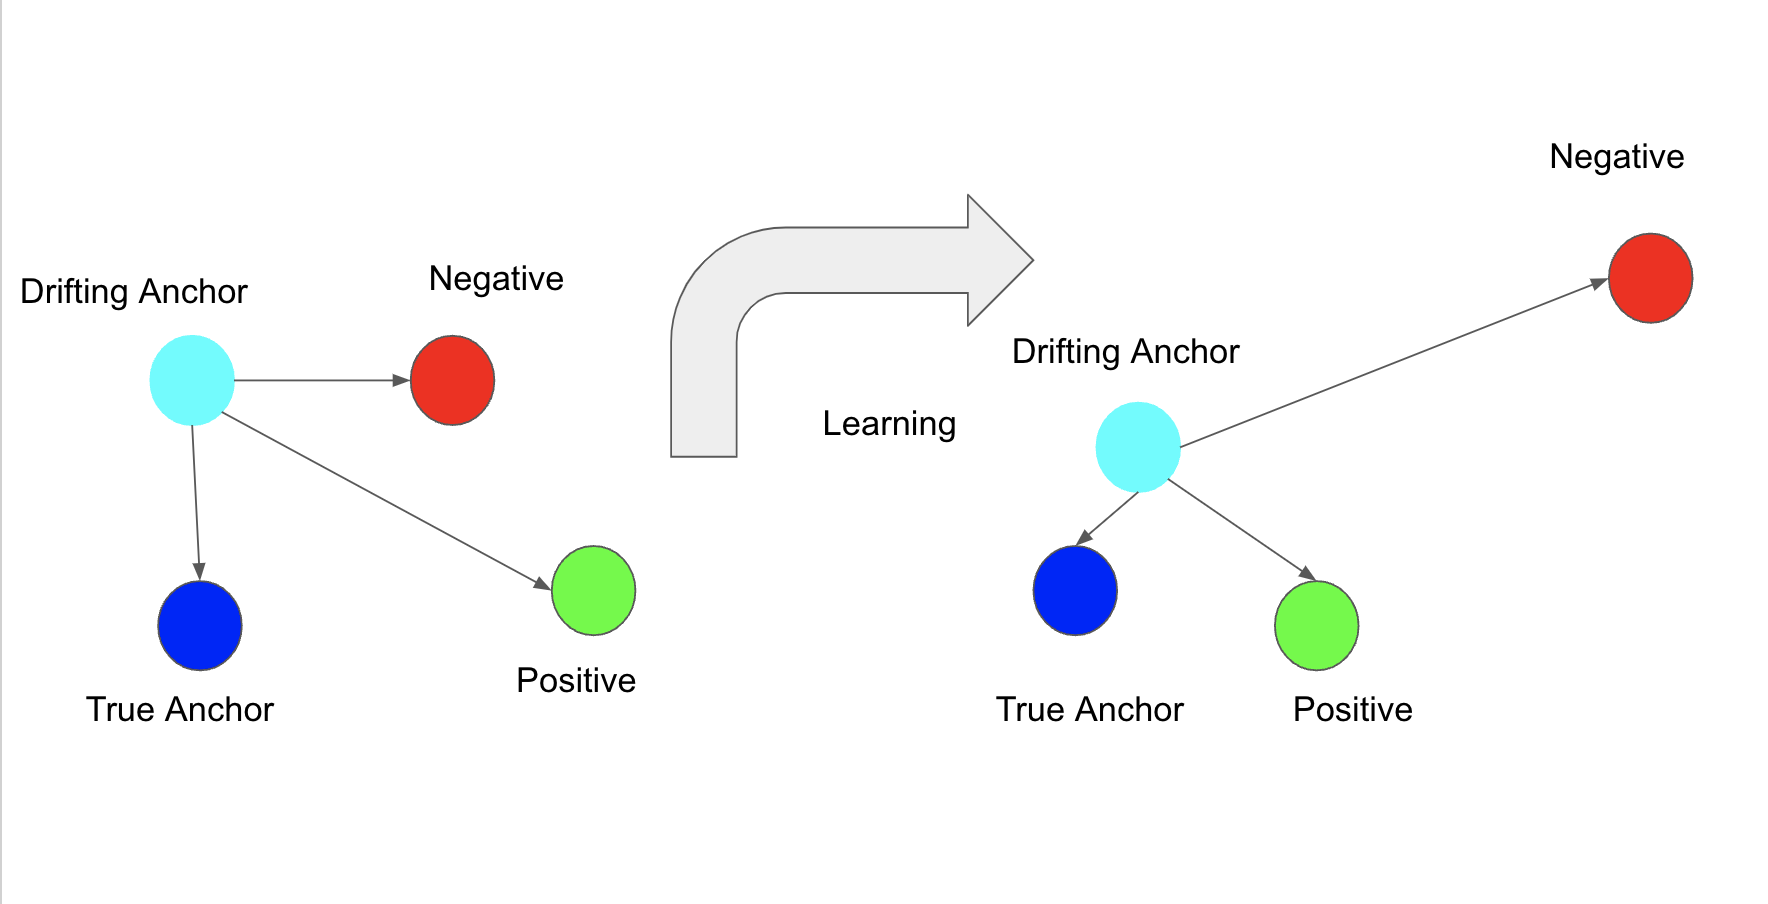
\includegraphics[width=\textwidth]{media-search/capot-figure1.png}}
  \caption{In order for the query encoder to represent noisy input in a close vector space we use contrastive learning to allow the model to learn to represent noisy queries to unaltered queries. Since the query encoder is trained without the passage encoder or notions of relevance, we use a notion of a fixed anchor to ensure the more robust query encoder approximates the original model with a drifting anchor, which is its representation for the non-noisy query.}
  \label{fig:capot-fig1}
\end{figure}
While neural methods clearly excel on the well formulated academic benchmarks, when faced domain shifts or queries with misspellings or typos, performance falters. On recent benchmarks like BEIR \cite{Thakur2021BEIRAH} cross-encoders have been shown to be more robust to shifts in domain than bi-encoders. When looking at queries that have some form of noise like typos and misspellings, the same holds \cite{zhuang-zuccon-2021-dealing}. Despite their superior performance on noisy queries and domain shifts, cross-encoders inference requirements makes the too expensive to use at scale. Cross-encoders produce a relevance score for each query-document pair and as a result, the inference load for each query for a purely cross-encoder based system is exactly the size of the index $D$. Avoiding this inefficiency, bi-encoder's have emerged as a popular method for retrieval, particularly for candidate generation in multi stage ranking systems. Bi-encoders leverage a query model and document model which are trained to match their representations in a latent space. Since document representations are query independent, they only need to be generated once and the inference load is limited to a single run of the query encoder. \\
Research on bi-encoder has been driven by the availability of large training datasets such as MS MARCO \cite{Campos2016MSMA}, Natural Questions (NQ)\cite{Kwiatkowski2019NaturalQA}, and Trivia QA (TQA) \cite{Joshi2017TriviaQAAL} . These datasets have allowed deep explorations on how to improve training procedure \cite{Qu2021RocketQAAO}, decrease index size \cite{Yamada2021EfficientPR} and model efficiency \cite{Khattab2020ColBERTEA}.  Despite the tremendous success,these neural methods models have been shown to be brittle to subtle shifts of search domain and minor variations in query formulation.  \\
Sidiropoulos et al. '22 \cite{Sidiropoulos2022AnalysingTR} and Zhuang et al. '21 \cite{zhuang-zuccon-2021-dealing} showed that dual encoders are quite brittle to typos but simple methods like data augmentation and contrastive learning can be implemented to improve performance on noisy queries. While methods like these help query encoders they are not without problems. Data augmentation introduces substantial overhead during training, requires complete model retraining when a new form of noise is discovered, and requires a new index to be generated. As a result, while data augmentation is effective, it may not be applicable to diverse training regimes and is at odds with the consistent growth in dataset and specialized training methods such as curriculum learning \cite{Mao2022CurriculumCC} and topic aware sampling \cite{Hofsttter2021EfficientlyTA}. \\
\begin{table}[htb!]
    \scalebox{0.55}{
    \begin{tabular}{|l|l|l|l|}
    \hline
        Noising Function & Alteration Type & Original & Alteration \\ \hline
        Determiner & Syntactic & who sang waiting for a girl like you & who sang waiting a a girl like you \\ \hline
        Synonym & Semantic & \makecell{Which was the first European country to \\ abolish capital punishment?} & \makecell{Which was the first European country \\ to abolish majuscule punishment?}\\ \hline
        Lemmatize & Syntactic & who plays young dr mallard on ncis & who play young dr mallard on ncis \\ \hline
        Stemming & Syntactic & who recorded the song still the one? & who record the song still the one? \\ \hline
        Random Character Swap & Surface & big little lies season 2 how many episodes & big litt e lies season 2 how many episodes \\ \hline
        Keyboard Character Swap & Surface & when did veterans day start being called veterans day & when djid veterans day start being called veterans day \\ \hline
        Character Delete & Surface & when did big air snowboarding become an olympic sport & when did big air snowboarding become an olympic sort \\ \hline
        Reorder Word & Surface & who is the main character in green eggs and ham & who is the main character and green eggs in ham \\ \hline
        Back-Translation & Semantic & what is project charter in project management & What is a project charter in project management \\ \hline
        Paraphrasing & Semantic & turkey and china time difference & \makecell{Time difference between Turkey and China in the middle \\ of the night, depending on the time difference.} \\ \hline
    \end{tabular}}
    \caption{Example of the forms of query noise that we leverage to evaluate how robust bi-encoders are to noise.}
    \label{tab:query-noise}
\end{table}
Seeking to improve performance on noisy queries without altering training regimes we introduce \textbf{C}onstrastive \textbf{A}llignment \textbf{PO}st \textbf{T}raining (CAPOT). CAPOT build on constrastive learning by training a model to learn that queries with noise (positive samples) should be closer to the anchor than unrelated queries. Unlike traditional constrastive learning, CAPOT introduces a notion of an anchoring loss between a drifting and fixed anchor. The fixed anchor is generated by extracting the query representation on a fixed encoder while the drifting anchor is based on the query representation the model learns. As the model learns query representation that groups noisy queries and their unaltered roots, we also constrain the models ability to alter the representation of the anchoring query, to avoid losses in relevance with the unaltered document encoder. To avoid complicated dual encoder training regimes CAPOT assumes that the document encoder and index are immutable and learn an improved query representation without altering existing relations to the index. \\
The main contributions of our work are as follows:
\begin{itemize}
\item We introduce benchmarks for noisy queries based on the popular MS MARCO, TriviaQA, and Natural Questions datasets, study the robustness of the current models, and show that they are all brittle and suffer from  
a sizable loss in accuracy on such data sets. 
\item We introduce CAPOT, a new efficient method for improving performance on noisy queries without retraining a model nor regenerating an index. 
\item We demonstrate that CAPOT is incredibly effective at making encoder robust, particularly with regard to typos. On our broad benchmarks, CAPOT approximates or exceeds the impact of data augmentation with the associated computational overhead.
\item We demonstrate that CAPOT is robust enough to prove functional with completely unsupervised data. Using the ORCAS dataset, CAPOT can approximate performance of Data Augmentation on NQ without access to the query distribution.
\end{itemize}
\section{Related Work}
\label{sec:rel}
\textbf{Bi-Encoders}, which are commonly called dual-encoders or dense retrievers, decompose ranking by leveraging the inner product of query and document representations to produce a relevance score for query document pairs. Since their document representations are query invariant, they can be pre-computed and loaded into an Approximate Nearest Neighbor (ANN) such as FAISS \cite{johnson2019billion} and at run time, for each query, the $k$ closest documents can be found with minimal latency. Since bi-encoders leverage LLM such as BERT \cite{Devlin2019BERTPO} they are often limited to ranking short passages of text and are commonly refereed to as Dense Passage Retrievers (DPR) \cite{Karpukhin2020DensePR}. Driven by their efficiency in deployment and relevance performance, DPR based models have rapidly become the building blocks for systems doing product search \cite{Magnani2022SemanticRA}, open domain question answering \cite{Karpukhin2020DensePR} and customer support \cite{Mesquita2022DenseTR}.\\
Recent work has heavily focused on improving the relevance of DPR models by improving the negative sampling using methods like ANCE \cite{Xiong2021ApproximateNN} and in-batch negatives \cite{Lin2021InBatchNF}. While effective DPR models are brittle to shifts in domain such that minor variations can cause a complete collapse in relevance. Li et al. '2022 introduced methods for improving such performance by having a single query encoder leverage multiple document encoders as a way of transferring between domains \cite{Li2022AnEA}. While effective, such a method caries a high computational load as multiple indexes must be maintained and updated. \\
\textbf{Data Augmentation} (DA) is a popular approach for improving how well models perform on new or noisy data. In data augmentation training is extending by augmenting the training data with modifications or perturbations which match the desired model behavior. DA is extremely common in computer vision where training data is commonly rotated, blurred,cropped, or zoomed-in/out \cite{Mikoajczyk2018DataAF} \cite{Zhong2020RandomED}. DA has become increasingly more popular in NLP and has been used to improve model performance \cite{Jiao2020TinyBERTDB}, simulate large scale training data when it is not available \cite{Li2020ADD}, and mitigate bias \cite{Lu2020GenderBI} in existing datasets. A detailed survey on DA approaches for NLP has been complied by Feng et al. 21' \cite{Feng2021ASO}.\\
\textbf{Contrastive Learning} builds on the notion of a contrastive loss \cite{Chopra2005LearningAS} which seeks to create clusters in the embedding space such that examples with a shared class are far from other classes but close to each other. Much like learning that queries with noise have a shared intent, Schroff et al. 15' leverage contrastive learning to to recognize faces despite different angles and perspectives \cite{Schroff2015FaceNetAU} by using a triplet loss. This approach is a natural fit for the world of search as relevance is at its core clustering relevant items close together and far from irrelevant items. Recently, constrastive learning has become a method for learning relevance at the corpora scale \cite{Xiong2021ApproximateNN} and for improving DPR on noisy queries \cite{Sidiropoulos2022AnalysingTR}.
\section{Are Query Encoders Robust to Noise?}
\label{create}
\begin{table*}[b!]
    \centering
    \scalebox{0.55}{
        \begin{tabular}{|l|l|l|l|l|l|l|l|l|l|l|}
    \hline
        Noise & seed 28026 & seed 28892 & seed 28984 & see 6870 & seed 31341 & median & stdev & CI & upper bound & lower bound \\ \hline
        No Noise & 0.324340 & 0.324063 & 0.323069 & 0.328069 & 0.320080 & 0.323924 & 0.002867 & 0.002513 & 0.326437 & 0.321411 \\ \hline
        Determiner & 0.258560 & 0.260123 & 0.255463 & 0.261204 & 0.257060 & 0.258482 & 0.002305 & 0.002020 & 0.260502 & 0.256462 \\ \hline
        Synonym & 0.207516 & 0.205220 & 0.203618 & 0.209447 & 0.205811 & 0.206322 & 0.002235 & 0.001959 & 0.208281 & 0.204363 \\ \hline
        Lemmatization & 0.315470 & 0.315402 & 0.315013 & 0.318352 & 0.310951 & 0.315038 & 0.002646 & 0.002320 & 0.317357 & 0.312718 \\ \hline
        Stem & 0.268777 & 0.270121 & 0.266453 & 0.272266 & 0.265884 & 0.268700 & 0.002633 & 0.002308 & 0.271008 & 0.266393 \\ \hline
        Random Character Swap & 0.168659 & 0.167019 & 0.164608 & 0.173576 & 0.168881 & 0.168549 & 0.003289 & 0.002883 & 0.171431 & 0.165666 \\ \hline
        Keyboard Character Swap & 0.159279 & 0.160566 & 0.156309 & 0.164849 & 0.158790 & 0.159959 & 0.003140 & 0.002752 & 0.162711 & 0.157207 \\ \hline
        Character Delete & 0.181659 & 0.179064 & 0.176293 & 0.184570 & 0.178657 & 0.180049 & 0.003164 & 0.002773 & 0.182822 & 0.177275 \\ \hline
        Word Reorder & 0.313691 & 0.312971 & 0.309866 & 0.313597 & 0.309563 & 0.311938 & 0.002051 & 0.001797 & 0.313735 & 0.310140 \\ \hline
        Back-Translation & 0.269536 & 0.265724 & 0.266155 & 0.271018 & 0.265379 & 0.267562 & 0.002548 & 0.002233 & 0.269795 & 0.265329 \\ \hline
        Paraphrase & 0.266934 & 0.265088 & 0.263751 & 0.267521 & 0.264953 & 0.265650 & 0.001546 & 0.001355 & 0.267005 & 0.264295 \\ \hline
        Average & 0.248584 & 0.247760 & 0.245509 & 0.251315 & 0.246001 & 0.247834 & 0.002316 & 0.002030 & 0.249864 & 0.245804 \\ \hline
    \end{tabular}}
    \caption{Unaltered Dense Model Performance on MSMARCO with regard to Mean Reciprocal Rank at 10.}
    \label{tab:msmarco-mrr10}
\end{table*}
While previous work has studied the impact of minor variations to queries such as typos and misspellings, query noise is much more diverse. Seeking to expand this understanding, we explore the impact of query alterations that evaluate surface, syntactic and semantic alterations. To apply noise to a query, we either edit a query to introduce a specific type of noise or we rewrite the query to simulate similarly worded intents. \\
For edited queries, an anchor word or character index is selected at random to be the noising index. Then, noise is applied either to the left, right, or at the noising index each with $\frac{1}{3}$ probability. For generated noise, a query is re-written leveraging a generative model. Since we are focused on evaluating how systems perform under moderate noise, we introduce each noising function independently and for edit-based methodologies, only perform a single word or character edit. An example for each kind of alteration can be found in table \ref{tab:query-noise}. \\

To study the impact of surface level alterations, we introduce noise in queries by simulating misspelling and typos by swapping, eliminating or shuffling characters in a query. To understand how systems may work when faced with natural shifts in keyword queries, we swap a word with another in the query by select two non-adjacent words at random. To understand how models respond to typos or character omissions we delete a character, inject a random character, or simulate a keyboard based typo by injecting a character close to its neighbor on a keyboard. \\ 
To study syntactic alterations we introduce noise which alters the syntax of the query introducing lemmas, stems, and determiners. Determiners are introduced in a similar fashion to typos. A word index is selected at random and a determiner is injected left,right, or at the word index. For stemming and lemmatization we leverage the NLTK toolkit \cite{bird2009natural} for our list of determiners, its lemmatizer and its porter stemmer. While we noise queries we select up to five random indexes to attempt stemming/lemmatization. Its worth noting that many queries do not have either stemmed or lemmatized version and as a result are un-noised. \\
To study semantic alterations we rewrite queries leveraging paraphrasing, back-translation, and synonyms. To introduce synonyms we select a word in a query and leverage NLTK's interface with WordNet \cite{Fellbaum2000WordNetA} to rewrite the query with an exact synonym. To paraphrase we rewrite queries using a T5 \cite{Raffel2020ExploringT} which has been fine-tuned on the PAWS \cite{Zhang2019PAWSPA} dataset. For back-translation use OpenNMT's \cite{klein-etal-2017-opennmt} machine translation models to translate queries from English to German and then from German to English. Its worth noting that these semantic noising methods are the most likely to alter the true query intent as can be seen by the 'hallucinations' seen in table \ref{tab:query-noise} paraphrase alteration. \\
Using the aforementioned noising approaches, we noise the queries on the MS MARCO passage ranking dataset \cite{Campos2016MSMA}, Natural Questions Passage ranking dataset \cite{Kwiatkowski2019NaturalQA} and the Trivia QA Passage Ranking dataset \cite{Joshi2017TriviaQAAL} to produce 3 query noise benchmarks. We release each dataset along with benchmark dense retrieval models to allow further  continued research on the subject. \\
\subsection{Baseline Model Training}
\begin{table}[h!]
    \centering
    \scalebox{0.7}{
    \begin{tabular}{|c|c|c|c|c|} \hline
        Dataset & Batch Size & Learning Rate & Train Length & Negative Passage \\ \hline
        NQ & 128 & 1e-5 & 40 & 1  \\ \hline
        TrivaQA & 128 & 1e-5 & 40 & 1 \\ \hline
        MSMARCO & 8 & 5e-6 & 3 & 8 \\ \hline
    \end{tabular}}
    \caption{Model Training parameters across tasks. NQ and TriviaQA are trained using 4 V100s while MSMARCO uses a single V100}
    \label{tab:params}
\end{table}
To ensure we understand how well trained dense retriever perform on noisy queries, we train a set of benchmarks not suited for noisy queries. We train a series of task specific bi-encoders leveraging the open source bi-encoder focused library Tevatron \cite{Gao2022TevatronAE}. For NQ and trivia QA we train on four V100 GPUs for about 5 hours while for MSMARCO we train on a single V100 GPU for 12 hours. Each bi-encoder uses a pre-trained BERT \cite{Devlin2019BERTPO} model for its initialization. Our query and document representation size is 768 dimensions and based on the last hidden representation of the CLS token without any additional linear projection. Further Details about training hyperparameters by task can be found in Table\ref{tab:params}. Each model is trained using 5 different random seeds with fixed optimal hyperparamers and we report the median score across the set of experiments. After training, we evaluate models by performing retrieval on a noised version of the intended dev/test split against the existing relevance labels. For all of our experiments we leverage untied bi-encoders as it allows us to optimized the query and passage encoder separately. We did explore experiments with tied encoders but they were unsuccessful as the document representation drifted along with the query representation. For experimental metrics we focus on recall accuracy at k with $k={20,100,200}$. Averaged results for bi-encoder can be found in table \ref{tab:bi-encoder-noise} and detailed results for MS MARCO with recall size 10 can be found in Table \ref{tab:msmarco-mrr10}, further detailed results in the appendix in the appendix. \\
\begin{table}[t!]
    \centering
    \scalebox{0.7}{
        \begin{tabular}{|l|l|l|l|l|l|l|l|l|l|}
    \hline
         Dataset & Acc @ 20 & with noise & Loss & Acc @ 100 & Acc with noise & Loss & Accy @ 200 & with noise & Loss \\ \hline
        NQ & 0.7973 & 0.7156 & -10.28\% & 0.8598 & 0.8158 & -5.12\% & 0.8825 & 0.8391 & -4.91\% \\ \hline
        MS Marco & 0.7163 & 0.5665 & -20.92\% & 0.8879 & 0.7491 & -15.63\% & 0.9378 & 0.7935 & -15.38\% \\ \hline
        TriviaQA & 0.7940 & 0.5665 & -4.90\% & 0.8501 & 0.8248 & -2.97\% & 0.8666 & 0.8472 & -2.24\% \\ \hline
    \end{tabular}}
    \caption{Retrieval accuracy (Acc) at K for Bi-encoders on unaltered and noisy queries. As recall set size grow, the impact of noise is greatly reduced. We find a large variation in impact of noise across datasets as the factoid queries from Trivia QA impacted $\frac{1}{5}$ to $\frac{1}{8}$ that of the web search queries of MS MARCO}
    \label{tab:bi-encoder-noise}
\end{table}
When observing the results, we find that our experiments align with prior research showing that dense retrieval methods are heavily susceptible to surface level variations such as typos. Methods which perform character level alterations on average see 50\% higher loss in accuracy than other methods. This large gap can be attributed to the vocabulary construction method of BERT and BERT like models where a minor alteration to a single character can produce large variations to tokenization. Taking a deeper look at the impact of noise, we find there is a non-uniform impact across datasets. The long, trivia-inspired queries of Trivia QA see minor losses in accuracy when compared to the real world web search queries of MSMARCO, up to $\frac{1}{8}$ the impact. Another finding is that the impact of noise is greatly reduced by increasing the size of the recall set. Across tasks and datasets increasing the recall set from 20 to 200 decreases the impact to accuracy by about 50\%. This leads us to believe that in the absence of data augmentation or post training optimization the clearest way to make dense retrieval robust to noise is to expand the recall set and allow cross encoders to re-rank the expanded results. Focusing on MSMARCO and its official recall metric of Mean Reciprocal Rank at depth 10 we see nearly a 50\% loss, Dropping from 0.324 to 0.159, on queries that have some form of typo. We believe these results not only motivate work on improving how robust dense retrieval are but highlight the importance of multi stage ranking. When exclusively reliant on dense retrieval methods the rankings are not robust to noise. However, if a bi-encoder is used for candidate generation and the recall set size is grown to 100 or 200, the impact to accuracy is no longer catastrophic.  
\section{Constrastive Alignment}
\subsection{Motivation}
A robust query encoder seeks to be able to represent queries that have a shared intent in a common latent space such that minor variations in the formulation of the intent lead to similar document ranking. Prior work has shown that data augmentation is effective method of increasing model robustness but it is not without cost. Data augmentation requires changes to existing training methodologies and complete regeneration of the passage index. Given that the generation of the passage index can take longer than it does to train the model \cite{Karpukhin2020DensePR} regenerating a new index and retraining a model every time a novel for of noise is discovered is not tractable. Besides its high cost in regenerating indexes, data augmentation increases training time by a factor of $n$ where $n$ is the number of augmentations used. Given our noisy queries, data augmentation causes a ten times longer training regimes and has no clear way to combine augmentation with topic aware sampling or curriculum learning. Motivated by this bottleneck, we introduce CAPOT, a new methodology for increasing model robustness which is \textbf{computationally inexpensive}, \textbf{independent of training} and as effective as augmentation. CAPOT works well because it is able to focus on improving the query encoder and leverages the short nature of queries to scale to large batch sizes.  \\
\subsection{CAPOT}
\textbf{C}ontrastive \textbf{A}lligment \textbf{Po}st \textbf{T}raining (CAPOT) is an expansion on traditional contrastive learning focused on making dual encoders robust to noise. The approach builds on the traditional triplet contrastive loss \cite{Schroff2015FaceNetAU} shown in equation \ref{eq:1} where $f$ is the model we are training, $x$ is the original anchor query, $x^+$ is a query where noise has been introduce and $x^-$ is a negative query selected at random.\\
\begin{equation} \label{eq:1} 
\begin{split}
    \Lagr_{triplet}(x, x^+, x^-) &= \sum_{x \in X} \max(0,\mathrel{\Vert} f(x) - \\
    & f(x^+) \mathrel{\Vert}_2^2 - \mathrel{\Vert} f(x) - f(x^-) \mathrel{\Vert}_2^2 + \epsilon)
\end{split}
\end{equation}
Based on the sensitivity seen to variations in positive and negative sample we introduce a modification to the triplet loss as shown in \ref{eq:2}. This modification controls the importance of the positive and negative components of the triplet loss to allow dataset specific tuning. In our experiments we find the ability to tune $\tau_{positive}$ and $\tau_{negative}$\ is crucial for optimizing performance and our optimal parameters can be found in table \ref{tab:param-capot}. \\
\begin{table}[b!]
    \centering
    \scalebox{0.9}{
        \begin{tabular}{|l|l|l|l|l|l|l|l|l|}
    \hline
        Dataset & Learning Rate  & $\tau_{positive}$ & $\tau_{negative}$ &  $\tau_{anchor}$ &  $\tau_{ranking}$ & Batch Size & Training Time \\ \hline
        NQ &  5.00E-05 & 2 & 0.2 & 2 & 0.7 & 2048 & 1 hour \\ \hline
        TriviaQA &  5.00E-05 & 1 & 0.1 & 2 & 1 & 2048 & 1.5 hours\\ \hline
        MS MARCO & 5.00E-05 & 1 & 0.1 & 2 & 1 & 2048 & 5 hours \\ \hline
    \end{tabular}}
    \caption{CAPOT optimal hyperparameters across datasets. Models were generally trained for 10 epochs but we find that a single epoch can provide 95\% of the final increase in performance.}
    \label{tab:param-capot}
\end{table}
\begin{equation} \label{eq:2} 
\begin{split}
    \Lagr_{triplet_\tau}(x, x^+, x^-) &= \sum_{x \in X} \max(0, \tau_{positive}*\mathrel{\Vert} f(x) - f(x^+) \mathrel{\Vert}_2^2 \\ 
    &- \tau_{negative}*\mathrel{\Vert} f(x) - f(x^-) \mathrel{\Vert}_2^2 + \epsilon_{triplet_{\tau}})
\end{split}
\end{equation}
While the use of the triplet loss can help our model learn to represent queries and noisy queries in a similar latent space it has the unwanted side effect of altering all other representations. In our early experiments the drift between an altered query encoder and the document encoder caused complete collapse in ranking ability. To avoid such a collapse we introduce an anchoring loss as shown in equation \ref{eq:3} where $f$ is the model we are training and $f_a$ is a copy at that model which is frozen at initialization. The anchoring loss is key to CAPOT as it allows us to optimize the query encoder without the document encoder as it allows us to constrains how much the model can drift.  \\
\begin{equation} \label{eq:3} 
    \Lagr_{anchor}(x) = \sum_{x \in X} \max(0,\mathrel{\Vert} f(x) - f_a(x) \mathrel{\Vert}_2^2 + \epsilon_{anchor})
\end{equation}
Finally, we leverage a ranking loss as shown in \ref{eq:4} between the anchored model $f_a$ and $f$ where we the model learns that $f(x^+)$ always rank higher than $f_a(x)$. While this component of the loss is not crucial we find we can leverage this to improve model performance slightly. \\

\begin{equation} \label{eq:4} 
    \Lagr_{ranking}(x^+, x^-) = \sum_{x \in X} \max(0,-y * (f(x^+)-f(-x) + \epsilon_{ranking})
\end{equation}
Using these three components, we combine each loss and its temperature control to produce the CAPOT loss shown in equation \ref{eq:5}.
\begin{equation} \label{eq:5} 
\begin{split}
    \Lagr_{CAPOT}(x, x^+, x^- ) &= \sum_{x \in X} \tau_{triplet} * \Lagr_{triplet} \\
    &+ \tau_{anchor} *  \Lagr_{anchor} + \tau_{ranking} * \Lagr_{ranking} 
\end{split}
\end{equation}
\section{Experimental Results}
\begin{table}[b!]
    \centering
    \scalebox{0.8}{
    \begin{tabular}{|l|l|l|l|l|l|l|}
    \hline
        Noise Type & Unaltered & Impact & Data Augmentation & impact & CAPOT & impact \\ \hline
        No Noise & \textbf{0.8501} & \textbf{0.00\%} & 0.8293 & -2.45\% & 0.8485 & -0.19\% \\ \hline
        Determiner & 0.8383 & -1.38\% & 0.8171 & -3.88\% & \textbf{0.8425} & \textbf{-0.90\%} \\ \hline
        Synonym & 0.8239 & -3.08\% & 0.8078 & -4.97\% & \textbf{0.8312} & \textbf{-2.23\%} \\ \hline
        Lemmatize & 0.8481 & -0.23\% & 0.8285 & -2.54\% & \textbf{0.8493} & \textbf{-0.10\%} \\ \hline
        Stem & 0.8436 & -0.77\% & 0.8267 & -2.75\% & \textbf{0.8482} & \textbf{-0.22\%} \\ \hline
        Random Character Swap & 0.8095 & -4.77\% & 0.8123 & -4.44\% & \textbf{0.8372} & \textbf{-1.52\%} \\ \hline
        Keyboard Character Swap & 0.8116 & -4.53\% & 0.8129 & -4.38\% & \textbf{0.8395} & \textbf{-1.25\%} \\ \hline
        Character Delete & 0.8133 & -4.33\% & 0.8119 & -4.49\% & \textbf{0.8375} & \textbf{-1.48\% }\\ \hline
        Reorder Word & 0.8299 & -2.37\% & 0.8256 & -2.88\% & \textbf{0.8486} & \textbf{-0.18\%} \\ \hline
        Back Translation & \textbf{0.8060} & \textbf{-5.19\%} & 0.7824 & -7.97\% & 0.8016 & -5.70\% \\ \hline
        Paraphrasing &\textbf{ 0.8240} & \textbf{-3.07\%} & 0.7980 & -6.13\% & 0.8229 & -3.20\% \\ \hline
        Average & 0.8248 & -2.97\% & 0.8123 & -4.44\% & \textbf{0.8358} & \textbf{-1.68\%} \\ \hline
        Typos & 0.8115 & -4.54\% & 0.8124 & -4.44\% & \textbf{0.8381} & \textbf{-1.42\%} \\ \hline
    \end{tabular}}
    \caption{Performance at depth 100 of models on all forms of noise on the TriviaQA dataset. Constrastive alignment out performs other methods on all forms of noise except for the semantic noise of paraphrasing and back translation.  }
    \label{tab:top-100-trivia-all}
\end{table}
To explore how well CAPOT works and how it compares to data augmentation, we evaluate these optimized models on the same noisy query datasets from our earlier experiments. For each dataset we train a set of models using data augmentation and we align our unaltered models using CAPOT and we report the median score of five runs. \\
Our data augmentation approach leverages the same training flow as our unaltered bi-encoder but we augment the training corpus by a factor of ten using our aforementioned noising approaches. After models are trained with data augmentation, we regenerate the passage index and perform fresh evaluation across the noisy query benchmarks. Looking at some performance metrics in table \ref{tab:top100-typo} we can see how effective this simple technique as its able to recover over 5\% of performance on the NQ dataset. However, looking at the performance on MS MARCO dataset, we can see that data augmentation does not always lead to an improvements in performance. On the noisy MS Marco dataset data augmentation methods are out performed by the unaltered bi-encoder model. We attribute this to the already noisy distribution of queries found in the MS Marco dataset. Since its queries come from a commercial search engine, they feature variations in spelling and representations which our noising approaches seek to emulate.\\
To find the optimal parameters for CAPOT we iterate over each portion of the $\Lagr_{CAPOT}$ sequentially. First, we find cosine distance between representations to be the only effective method of aligning representations. Next, since we have 10 types of noise, we iterate hyperparamets based on model recovers accuracy on the un-noised input the best. This approach allows us to find the parameters specified in table \ref{tab:param-capot}. Additionally we experiment with the use of hard-negatives and in batch negatives but we do not find any noticeable improvement. \\
Our constrastive alignment approach takes advantage of training on only query encoder and fixing the document encoder. Since the average query length for each our our datasets is shorter than BERT's context window we train with a max sequence length of 28. This allows us to scale to an effective batch size of 2048. This large batch size means training is incredibly quick and effective as a full alignment run on the NQ dataset takes a single hour while the use of data augmentation requires 26 hours for training and an additional day for index generation. Additionally, by fixing the passage encoder during alignment, we can focus on improving model performance without altering complicated training methods like curriculum learning or topic aware sampling. If these approaches are used they can be applied prior and independently to alignment which is not the case for augmentation. \\ 
\begin{table}[htb!]
    \centering
        \begin{tabular}{|l|l|l|l|}
    \hline
        Dataset & Baseline & Data Augmentation & CAPOT \\ \hline
        NQ & 0.7871 & \textbf{0.8392} & 0.8352 \\ \hline
        TriviaQA & 0.8115 & 0.8124 & \textbf{0.8436} \\ \hline
        MS Marco & 0.5868 & 0.5887 & \textbf{0.7245} \\ \hline
    \end{tabular}
    \caption{Performance at Depth 100 of models on noisy queries focused on character based surface level alterations (typos). We note that on the natural questions dataset data augmentation slightly exceeds CAPOT and on all other datasets CAPOT exceed by a significant margin}
    \label{tab:top100-typo}
\end{table}

\begin{table}[htb!]
    \centering
        \begin{tabular}{|l|l|l|l|}
    \hline
        Dataset & Baseline & Data Augmentation & CAPOT \\ \hline
        NQ & 0.8158 & \textbf{0.8369} & 0.8300 \\ \hline
        TriviaQA & 0.82482 & 0.8123 & \textbf{0.8358} \\ \hline
        MS Marco & 0.7345 & 0.6314 & \textbf{0.7393} \\ \hline
    \end{tabular}
    \caption{Performance at depth 100 of model on the average of all forms of noise. Despite careful tuning on the MSMARCO dataset neither data augmentation nor CAPOT highly outperform the unaltered model. We attribute this to the size and real world query provenance of the dataset. }
    \label{tab:top-100-average}
\end{table}
\begin{table}[ht!]
\centering
    \scalebox{0.8}{
        \begin{tabular}{|l|l|l|l|l|l|l|}
    \hline
        Noise Type & Unaltered & impact & Data Augmentation & impact & CAPOT & impact \\ \hline
        No Noise & \textbf{0.8879} & \textbf{0.00\%} & 0.7183 & -19.10\% & 0.7970 & -10.24\% \\ \hline
        determiner & \textbf{0.7766} & \textbf{-12.54\%} & 0.6302 & -29.02\% & 0.7699 & -13.29\% \\ \hline
        synonym & \textbf{0.6809} & \textbf{-23.31\%} & 0.5501 & -38.04\% & 0.6196 & -30.21\% \\ \hline
        lemmatize & \textbf{0.8754} & \textbf{-1.41\%} & 0.7173 & -19.21\% & 0.8087 & -8.92\% \\ \hline
        stem & \textbf{0.7930} & \textbf{-10.69\%} & 0.6805 & -23.36\% & 0.7923 & -10.77\% \\ \hline
        Random Character Swap & 0.5800 & -34.68\% & 0.5881 & -33.76\% & \textbf{0.7236} & \textbf{-18.50\%} \\ \hline
        Keyboard Character Swap & 0.6197 & -30.21\% & 0.5903 & -33.52\% & \textbf{0.7299} & \textbf{-17.79\%} \\ \hline
        Character Delete & 0.6197 & -30.21\% & 0.5877 & -33.81\% &  \textbf{0.7199} & \textbf{-18.92\%} \\ \hline
        Reorder Word & 0.8757 & -1.37\% & 0.7074 & -20.32\% & 0.8348 & -5.98\% \\ \hline
        BackTranslation & 0.7860 & -11.47\% & 0.6249 & -29.62\% & 0.6891 & -22.39\% \\ \hline
        paraphrase & 0.7967 & -10.27\% & 0.6374 & -28.21\% & 0.7057 & -20.52\% \\ \hline
        Average & 0.7345 & -17.28\% & 0.6314 & -28.89\% & 0.7394 & -16.73\% \\ \hline
        Typos & 0.5868 & -33.91\% & 0.5887 & -33.70\% & 0.7245 & -18.40\% \\ \hline
    \end{tabular}}
    \caption{Performance of Modeling approaches at depth 20 on the TriviaQA dataset.}
    \label{tab:msmarco-full}
\end{table}
\section{Expanding Contrastive Alignment}
\begin{table}[htb!]
    \centering
    \scalebox{0.65}{
    \begin{tabular}{|l|l|l|l|l|l|l|l|l|}
    \hline
        Noise Type & Unaltered & Impact & CAPOT MLM & Impact & CAPOT-TriviaQA & Impact & CAPOT-ORCAS & Impact \\ \hline
        No Noise & 0.7940 & 0.00\% & 0.7352 & -7.41\% & 0.7853 & -1.10\% & 0.7673 & -3.36\% \\ \hline
        determiner & 0.7736 & -2.57\% & 0.7154 & -9.90\% & 0.7776 & -2.07\% & 0.7604 & -4.24\% \\ \hline
        synonym & 0.7511 & -5.41\% & 0.6917 & -12.89\% & 0.7597 & -4.33\% & 0.8123 & 2.31\% \\ \hline
        lemmatize & 0.7906 & -0.43\% & 0.7341 & -7.54\% & 0.7869 & -0.90\% & 0.7695 & -3.09\% \\ \hline
        stem & 0.7821 & -1.50\% & 0.7257 & -8.60\% & 0.7824 & -1.46\% & 0.7668 & -3.42\% \\ \hline
        Random Character Swap & 0.7264 & -8.51\% & 0.6760 & -14.86\% & 0.7674 & -3.35\% & 0.7583 & -4.49\% \\ \hline
        Keyboard Character Swap & 0.7234 & -8.89\% & 0.6787 & -14.52\% & 0.7690 & -3.15\% & 0.7562 & -4.76\% \\ \hline
        Character Delete & 0.7314 & -7.88\% & 0.6786 & -14.53\% & 0.7647 & -3.69\% & 0.7528 & -5.19\% \\ \hline
        Reorder Word & 0.7805 & -1.70\% & 0.7280 & -8.31\% & 0.7874 & -0.83\% & 0.7681 & -3.27\% \\ \hline
        BackTranslation & 0.7405 & -6.74\% & 0.6813 & -14.19\% & 0.7356 & -7.35\% & 0.7148 & -9.97\% \\ \hline
        paraphrase & 0.7510 & -5.41\% & 0.6866 & -13.52\% & 0.7419 & -6.56\% & 0.7195 & -9.38\% \\ \hline
        Average & 0.7551 & -4.90\% & 0.6996 & -11.89\% & 0.7673 & -3.37\% & 0.7579 & -4.55\% \\ \hline
        Typos & 0.7271 & -8.43\% & 0.6778 & -14.64\% & 0.7671 & -3.39\% & 0.7558 & -4.82\% \\ \hline
    \end{tabular}}
    \caption{Performance of Modeling approaches at depth 20 on the TriviaQA dataset.}
    \label{tab:ORCAS-aling}
\end{table}
Seeking to explore scalable contrastive alignment works we explore expansions to pre-training and to using unrelated training data. First, we generate a corpus of 10 million queries by extracting all unique queries from the ORCAS \cite{craswell2020ORCAS} click dataset. Using these queries, we create create positive and negative noisy samples using the same noising approach we have discussed prior. Using these 100m queries we evaluate how else constrastive alignment can be used. \\
To explorer contrastive alignment's ability to generate a generalizable robust retrieval model we align a model prior to retrieval specific training. In practice this means we perform alignment on a BERT model which is not fine-tuned for retrieval tasks. We train for a single epoch on the Noisy-ORCAS corpus using the $\tau_{positive}=1.0$,$\tau_{negative}=0.1$,and $\tau_{anchor}=1.0$ on 4 V100 GPUs with a batch size of 2048. Then, we leverage this optimized model as the initialization of our unaltered bi-encoder models training procedure. As shown in table \ref{tab:ORCAS-aling} this approach is nowhere as effective as alignment post training. In fact, the usage of this pre-trained model on average leads to twice the loss in accuracy on noisy queries as an unaltered BERT model.\\
To explore the impact of using CAPOT without access to the query distribution we perform alignment on a bi-encoder model trained for the TriviaQA using a portion of the Noisy-ORCAS data to perform alignment. We use the same hyperparameters as prior experiments but due to the size of the ORCAS data, limit training to 1 million samples. As shown in table \ref{tab:ORCAS-aling}, this approach improves performance relative to baseline but is unable to match the performance of aligning on the true query distribution. Despite aligning on un unrelated query set, using CAPOT on the noisy orcas dataset is able to reduce the impact of typos from 8.43\% to 4.82\% which leads us to believe this approach is an effective general approach for create typo robust query encoders. 
\section{Discussion}
Looking at the results in table \ref{tab:top-100-trivia-all} the effectiveness of CAPOT is immediately understandable. On the Trivia QA benchmark aligned models out perform all other methods by a sizable margin for all forms of noise but back translation and paraphrasing. Looking at the aggregate score shown in table \ref{tab:top100-typo} we can see that CAPOT is an incredibly effective way of create typo robust query representations. When queries have typos, CAPOT is able to outperform or match data augmentation performance despite its decreased computational overhead. When we look at performance on individual types of noise we find our method to not be as effective in improving the relevance of minor syntactic shifts such as lemmatization or stemming. We attribute this to the minor gap that is already seen when queries receive syntactic alteration which on datasets such as TriviaQA, causes under a 2\% loss in accuracy.\\
When we look at performance averaged across all types of noise as shown in table \ref{tab:top-100-average} we find that CAPOT is effective but no longer has as substantial improvements seen on queries with typos. The performance on MS Marco is particularly of note as CAPOT performance barely out performs the baseline model. Looking at detail results found in table \ref{tab:msmarco-full} we can see that despite massive improvements on queries with typos, CAPOT and data augmentation both double the loss of relevance on back-translation, stemming, and paraphrasing and 4-10x it on lemmatization. We attribute this impact to the relative importance on character level alterations our alignment dataset has. Three out of the 10 methods focus on learning alignments based around minor character shifts and as a result the performance optimizes there to the detriment of other forms of noise.   \\
A limitation of contrastive alignment is its ability to preserve accuracy on queries that have not received noise. On the NQ dataset, at depth 20, data augmentation sees accuracy drops are within the confidence internals of the baseline model while CAPOT models see a -2.37\% drop. We attribute this to the minor drift in representation the anchoring loss is unable fully optimize. \\
As a generalization, we find that neither data augmentation nor contrastive alignment has any relevance improvement for queries that have been paraphrased or back-translated. We believe this is because the query encoder is unable to learn a true query intent based latent representation for queries and as a result is unable to represent queries by intents. This makes us believe that neither data augmentation nor contrastive alignment are apt tools to learn intent based query representations without access to much larger datasets that group queries by intent such as web search logs used by the Generic Intent Representation of query vectors \cite{Zhang2019GenericIR}.\\
\begin{figure}[htb!]
    \centering
    \scalebox{0.5}{
    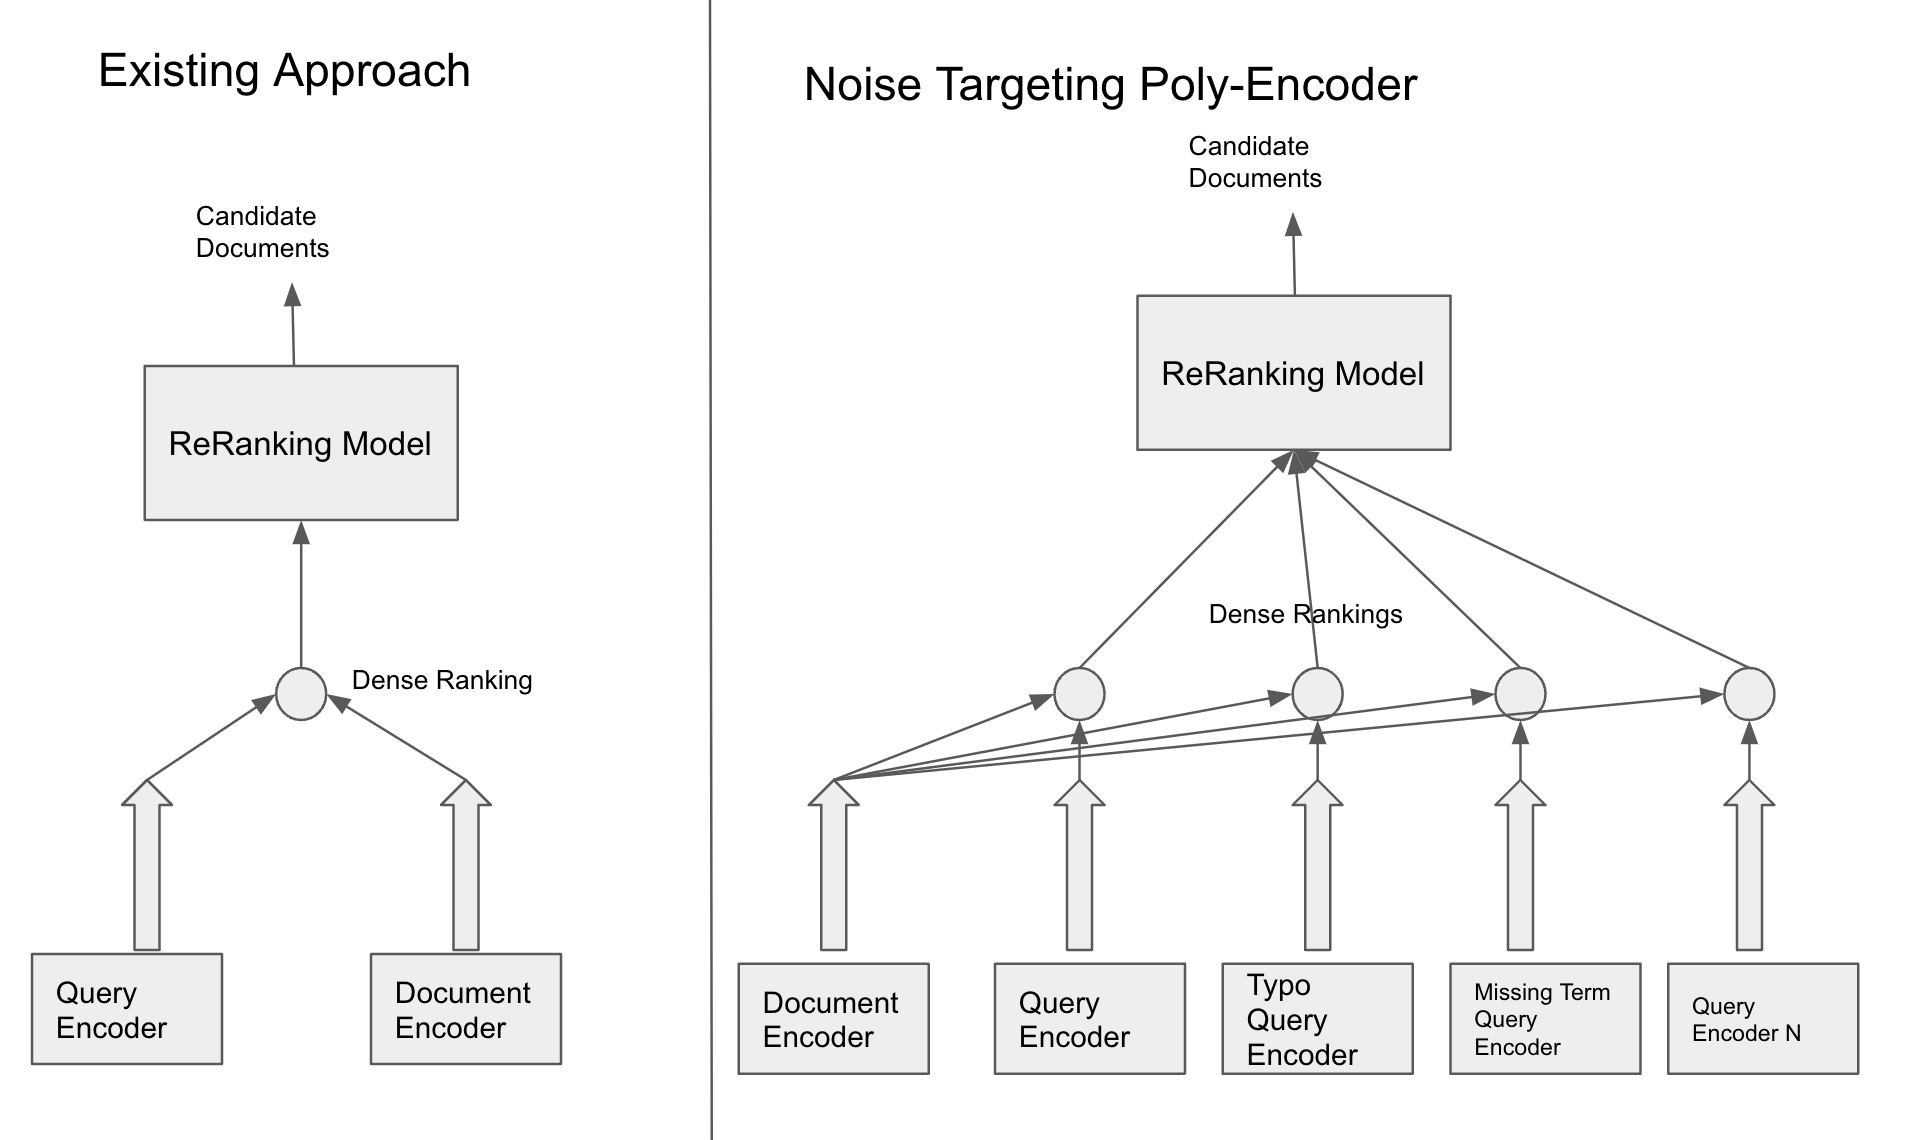
\includegraphics{media-search/capot-figure2.png}}
    \caption{Proposed poly-encoder architecture using noise targeted query encoders optimized with CAPOT}
    \label{fig:capot-fig2}
\end{figure}
The largest impact we see in using constrastive alignment is the ability to use constrastive augmentation to expand any existing bi-encoder into a poly-encoder. Contrastive alignment optimizes a query encoder given a fixed index and as a result it becomes possible to produce multiple specialized query encoders which interacts with one unaltered index. This ability to expand to a poly encoder means that when a deficiency is found in a bi-encoder, a specialized encoder can be created. Moreover, this novel noise optimized encoder can be used without any additional index generation and can be deployed in parallel  When bi-encoders are leveraged as candidate set generation tools the ability to   We believe the impact of CAPOT is that unlike Data Augmentation, Unlike data augmentation the CAPOT aligned encoder can be used as direct replacement or supplement to the existing query encoder. By combining an aligned encoder with a naive encoder, candidate generation can maximize recall and ensure performance on noisy queries. This constrastive alignment based poly encoder can be seen in figure \ref{fig:capot-fig2}. Instead of seeking to have a single query encoder that learns all surface and semantic forms of query representations we propose leveraging CAPOT to create a poly encoder of noise targeting query encoders. The associated re-ranking cost of 5 targeted encoders with set sizes of 20 is equal to that of expanding the initial candidate set size to 100. This approach allows 
\section{Conclusion}
In this work we have introduced a novel framework which increases performance on noisy queries for bi-encoder retrieval models. By extending the constrastive triplet loss with an anchoring loss CAPOT is able to improve performance without the need to retrain a model nor regenerate the index. To motivate our experimentation and quantify the impact of query noise we introduce three novel noisy retrieval datasets based on MS MARCO, TriviaQA and Natural questions finding traditional modeling approaches can see nearly 50\% loss in retrieval accuracy when a simple typo is present. Motivated by these results, we demonstrate the effectiveness of data augmentation and show how CAPOT's approximates or exceed it. Finally, we demonstrate how well  CAPOT works by approximating the performance of data augmentation while aligning the encoders on an the unrelated query distribution of the ORCAS dataset. \\
Building on the effectiveness of CAPOT in future work we will study how constrastive alignment can be used to compress retrieval models without having access to specialized and optimized training configurations. By using constrastive alignment post training we believe we can apply compression approaches like quantization, structured and unstructured prunning without having access to the training dataset nor methodology.  
\section{Current Work}
\subsection{Quick Dense Retrievers consume KALE: Post Training Kullback–Leibler Alignment of Embeddings for Asymmetrical dual encoders}
Bi-encoder based retrievers have becoming a dominant architecture for performing semantic retrieval at scale. While effective, bi-encoders commonly leverage a BERT based language model to generate query and document embeddings and as a result efficient inference at scale can be difficult. In our work we explore the role of asymmetry between the query and document models as a way of optimizing inference. Using a combination of asymmetrical training, structural pruning, and alignment of compressing encoding we are able to create models which can improve model inference with little to no loss in retrieval accuracy. As shown in table \ref{tab:search-asymetry} direct usage of decreased models lead to losses in accuracy such as the 13\% dip from a 12 layer model to a 3 layer model. However, if a model leverages asymmetrical training and then further compresses with post training alignment, it is possible to heavily improve model inference efficiency without major loss in accuracy. \\ 
When bi-encoder models are used in latency sensitive production workloads current approaches improve efficiency by using a compressed pre-trained language model like DistilBERT \cite{Sanh2019DistilBERTAD} or rely on post training structural pruning. As shown in figure \ref{fig:KALE-NQ-Top20}, \ref{fig:KALE-NQ-Top40}, \ref{fig:KALE-NQ-Top100},\ref{fig:KALE-NQ-Top200} using asymmetrical training and embedding alignment leads to major improvements in inference efficiency with the smallest losses in accuracy. Looking at figure \ref{fig:KALE-NQ-Top100} we can see that prior approaches require over $6\%$ loss in accuracy to achieve 4x improvement in efficiency while our methodology delivers the same inference efficiency improvements with less than 1\% loss in accuracy. 
\begin{figure}[!htb]
    \centering
    \scalebox{0.6}{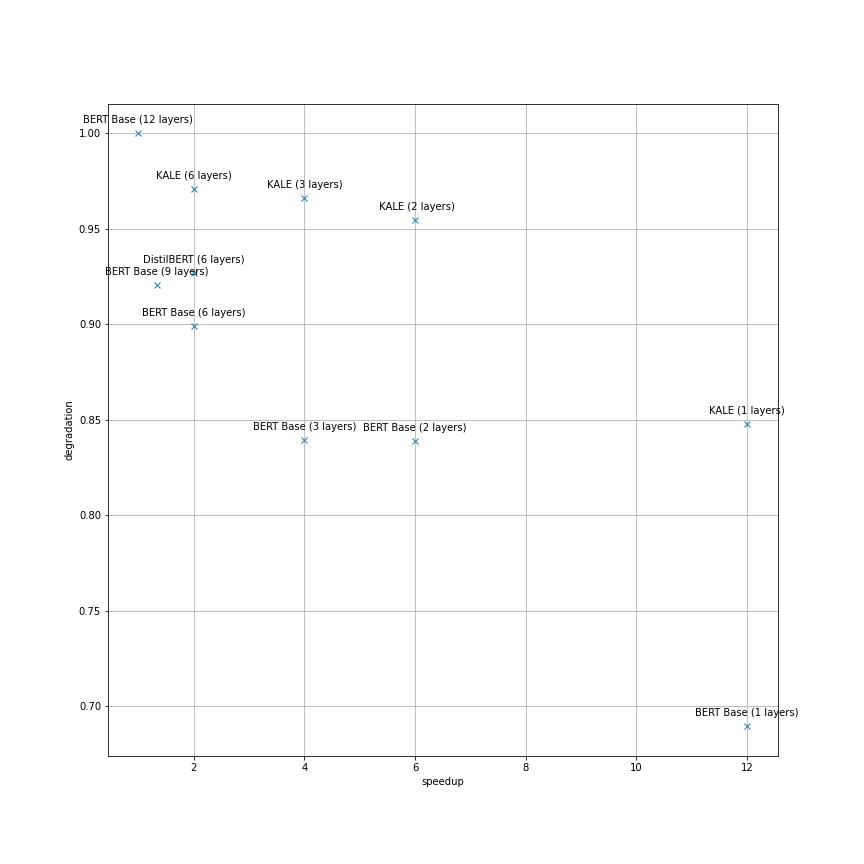
\includegraphics{media-search/KALE-NQ-20.png}}
    \caption{The trade off between inference speedup and recall degradation on the NQ passage retrieval dataset measuring the recall accuracy at 20. Using KALE allows for major improvements in inference speed without the sharp drop off in accuracy which is expected.  }
    \label{fig:KALE-NQ-Top20}
\end{figure}
\begin{figure}[!htb]
    \centering
    \scalebox{0.7}{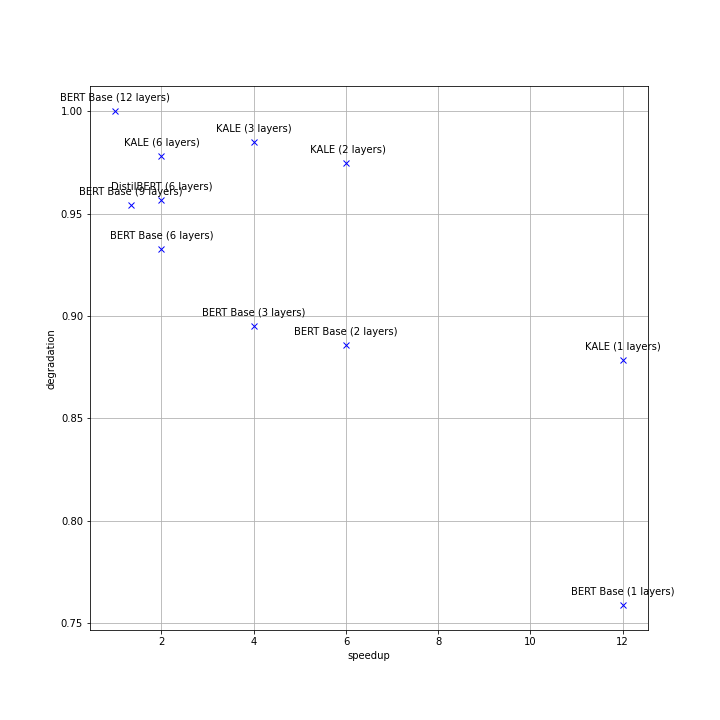
\includegraphics{media-search/KALE-NQ-40.png}}
    \caption{The trade off between inference speedup and recall degradation on the NQ passage retrieval dataset measuring the recall accuracy at 40. With an increased recall set size degradation's of accuracy are lessened.}
    \label{fig:KALE-NQ-Top40}
\end{figure}
\begin{figure}[!htb]
    \centering
    \scalebox{0.7}{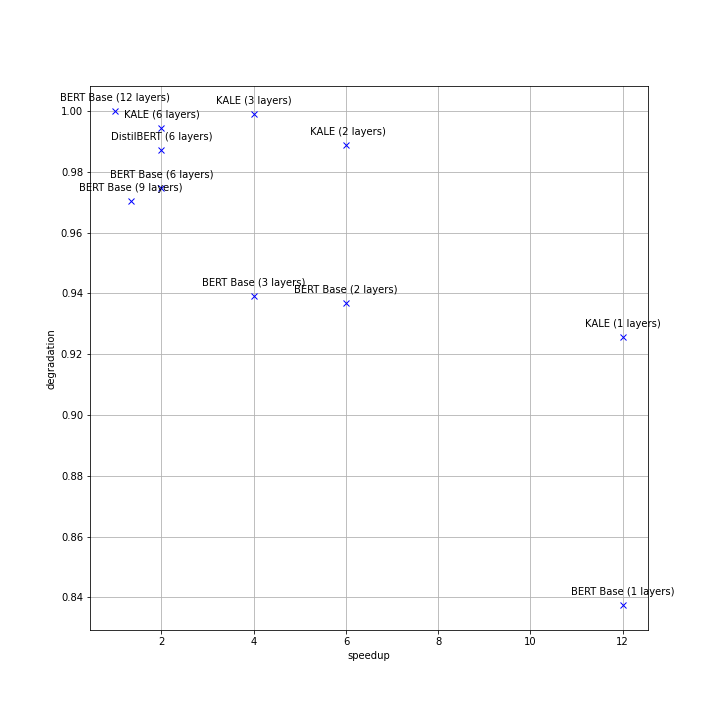
\includegraphics{media-search/KALE-NQ-100.png}}
    \caption{The trade off between inference speedup and recall degradation on the NQ passage retrieval dataset measuring the recall accuracy at 100. }
    \label{fig:KALE-NQ-Top100}
\end{figure}
\begin{figure}[!htb]
    \centering
    \scalebox{0.7}{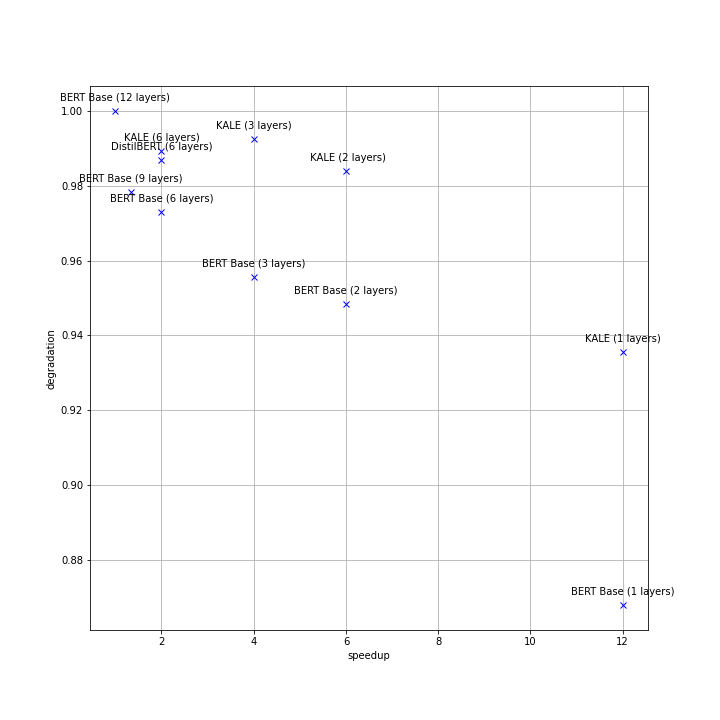
\includegraphics{media-search/KALE-NQ-200.png}}
    \caption{The trade off between inference speedup and recall degradation on the NQ passage retrieval dataset measuring the recall accuracy at 200. }
    \label{fig:KALE-NQ-Top200}
\end{figure}
\begin{table}[!htb]
    \centering
    \scalebox{0.8}{
    \begin{tabular}{|l|l|l|l|l|l|l|}
    \hline
        Model & Query Layers & Document Layers & Speedup & Acc @ 20  & Acc  @100 & Acc @ 200 \\ \hline
        BERT base uncased & 12 & 12 & 1x & 79.83 & 86.34 & 88.42 \\ \hline
        DistilBERT base uncased & 6 & 6 & 2x & 73.88  & 84.74 & 87.26 \\ \hline
        BERT base uncased & 3 & 3 & 4x & 66.92  & 80.61 & 84.49 \\ \hline
        BERT base uncased & 3 & 6 & 4x & 77.01  & 85.76 & 87.42  \\ \hline
        BERT base uncased & 2 & 6 & 6x & 76.09  & 84.88  &  87.01 \\ \hline
        BERT base uncased & 1 & 6 & 12x &  68.14 & 79.81 & 82.96 \\ \hline
    \end{tabular}}
    \caption{Impact of compression on inference speedup and retrieval recall accuracy (Acc) across model type. Leveraging asymmetrical bi-encoder training and post training alignment of pruned query encoders allows for 6x improvements in inference throughput with less than 2\% loss in accuracy on the NQ \cite{Kwiatkowski2019NaturalQA} passage retrieval task. When asymmetrical training is combined with post training structural pruning and embedding alignment a 2 layer query encoder out performs 6 layer distil BERT model despite being 3 times smaller.}
    \label{tab:search-asymetry}
\end{table}
\subsection{Leveraging Unstructured Sparsity for Efficient Dense Retrieval Serving}
Due to the widespread deployment of information retrieval workloads, inference typically happens without an accelerator like a GPU. To ensure that workloads which leverage language models can meet the stringent latency needs which are common to search, neural models commonly use structural compression to reach latency requirements despite losses in accuracy. In our work we have been actively combining unstructured sparsity, quantization and dense retrieval to create efficient bi-encoder inference on CPUs. Using a sparse aware inference run-time like DeepSparse \cite{deepsparse} or sparseDNN \cite{Wang2021SparseDNNFS} the use of sparsity can be used to improve the efficiency of model inference greatly. As shown in table \ref{tab:sparse-ir}, unstructured sparsity and quantization can be leveraged to improve model inference by 4x with less than 1\% loss in accuracy and 8x with less than 2\%.
\begin{table}[!htb]
    \centering
    \
    \begin{tabular}{|l|l|l|l|l|}
    \hline
        Sparsity & queries/Sec & Accuracy @ 20  & Accuracy @100 & Accuracy @ 200 \\ \hline
        0 & 80.55 & 79.83 & 86.34 & 88.42 \\ \hline
        90 & 332.31 & 78.78 & 85.84 & 87.70 \\ \hline
        80 4block (quantized) & 640.19 & 78.48 & 85.62 & 87.17 \\ \hline
    \end{tabular}
    \caption{Leveraging Sparsity and Quantization can improve the throughput of inference by 8 times with less than 2\% loss in accuracy on the NQ \cite{Kwiatkowski2019NaturalQA} passage retrieval task}
    \label{tab:sparse-ir}
\end{table}

\section{Experimentation Plan}
\scalebox{0.8}{
\begin{tabular}{r |@{\foo} l}
December 2022 & Write Up Leveraging Unstructured Sparsity for Efficient Dense Retrieval Serving\\
January 2023 & Write Up Quick Dense Retrievers Consume KALE: KL Asymmetrical Alignment of Encoders \\
\end{tabular}
}

\chapter{Scaling Multi-Lingual Classification and Abstractive Summarization to Web-Scale workloads}
\label{chp:Multi}
%\input{scaling-MT-AS}
\bibliographystyle{IEEE_ECE}
\bibliography{thesisrefs,anthology} 
\appendix
\label{chp:appendix}
\section{Introducing and Transferring Sparsity for efficient inference}
\label{app:sparsity}
\section{Robust and Efficient Semantic Retrieval}
\label{app:retrieval}

\section{Scaling Multi-Lingual Classification and Abstractive Summarization to Web-Scale workloads}
\label{app:scaling-workload}

\section{Publications}
\begin{itemize}
\item \href{https://arxiv.org/abs/2203.07259}{The Optimal BERT Surgeon: Scalable and Accurate Second-Order Pruning for Large Language Models} - Eldar Kurtic, \textbf{Daniel Campos}, Tuan Nguyen, Elias Frantar, Mark Kurtz, Benjamin Fineran, Michael Goin, Dan Alistarh - \href{https://2022.emnlp.org/}{EMNLP 2022}
\item \href{https://arxiv.org/abs/2205.12452}{Sparse*BERT: Sparse Models Generalize To New tasks and Domains} - \textbf{Daniel Campos}, Alexandre Marques, Tuan Nguyen, Mark Kurtz, ChengXiang Zhai - \href{https://www.sparseneural.net/}{Sparsity in Neural Networks Workshop at ICML 2022}
\item \href{https://arxiv.org/abs/2303.17612}{oBERTa: Improving Sparse Transfer Learning via improved initialization, distillation, and pruning regimes} - \textbf{Daniel Campos}, Alexandre Marques, Mark Kurtz, ChengXiang Zhai 
\item \href{https://arxiv.org/abs/2304.00114}{Dense Sparse Retrieval: Using Sparse Language Models for Inference Efficient Dense Retrieval} - \textbf{Daniel Campos}, ChengXiang Zhai
\item \href{https://arxiv.org/abs/2304.03401}{Noise-Robust Dense Retrieval via Contrastive Alignment Post Training} - \textbf{Daniel Campos}, Alessandro Magnani, ChengXiang Zhai
\item \href{https://arxiv.org/abs/2304.01016}{Quick Dense Retrievers Consume KALE: Post Training Kullback Leibler Alignment of Embeddings for Asymmetrical dual encoders} - \textbf{Daniel Campos}, Alessandro Magnani, ChengXiang Zhai
\item \href{https://arxiv.org/abs/2211.15927}{Compressing Cross-Lingual Multi-task Models at Qualtrics} - \textbf{Daniel Campos}, Daniel Perry, Samir Joshi, Yashmeet Gambhir, Wei Du, Zhengzheng Xing, and Aaron Colak - \href{https://aaai.org/Conferences/AAAI-23/iaai-23-call/}{The Thirty-Fifth Annual Conference on Innovative Applications of Artificial Intelligence (IAAI-23)}
\item \href{https://arxiv.org/abs/2304.02721}{To Asymmetry and Beyond: Structured Pruning of Sequence to Sequence Models for Improved Inference Efficiency} - \textbf{Daniel Campos}, ChengXiang Zhai
\end{itemize} 
\backmatter
\end{document}

